%!TEX root = ../phd-thesis-lei-ma.tex

\chapter{\label{chap:matter}Neutrino Oscillations with Oscillatory Matter Profiles}

In certain regions inside a star or a supernova where convection is prominent, the matter density varies rapidly as a function of distance~\cite{Muller2015, Couch2015}. The neutrino flavor evolution in such environments is qualitatively different than that with a smooth density profile~\cite{Krastev1989, Loreti1994,Akhmedov2000, Friedland2006,Kneller2010,Kneller2013,Patton2014}. For example, the flavor conversion of the neutrino is greatly enhanced if the matter density fluctuates with certain wave numbers. This is known as the parametric resonance~\cite{Krastev1989,Akhmedov1999}.

In this chapter, I will explain the parametric resonance from the perspective of Rabi oscillations. I will first review the Rabi oscillation phenomena and derive a criterion when the off-resonance Rabi mode may have a significant impact on the resonance behavior. I will then introduce the background matter basis where the equation of motion simplifies. After demonstrating the simplest example of the parametric resonance in the presence of a sinusoidal matter profile with the Rabi formula, I will explain the interference effect when there exist multiple Fourier modes in the matter profile. Finally I will show how to use the Jacobi-Anger expansion to decompose an arbitrary matter profile into an infinite sum of Rabi modes. This decomposition is similar to what J. Kneller et al. did in reference \cite{Kneller2013,Patton2014} but is achieved in a way that makes the physics much more transparent. I will also use the criterion that I have derived for the interference between two Rabi modes to show that only a finite number of Rabi modes are relevant in a real physical system.

% In Sec.~\ref{sec:jacobi} we discuss the technique of decomposing the neutrino flavor conversions into summation of Rabi oscillations, by applying a specific unitary transformation and the Jacobi-Anger expansion. As the system is exactly decomposed into multiple Rabi oscillations, we can interpret neutrino flavor oscillations in any matter density fluctuations, in principle. As an example, we solve the neutrino flavor transitions in a castle wall matter profile, which contains infinite frequencies from the aspect of Fourier series. Finally I will discuss an algorithm to select the Fourier modes of a matter profile that have the largest impact on the flavor conversion of the neutrino.



% \section{\label{chap:basics-section:astro}Stars as Neutrino Factories}


% In the following sections of this chapter, I will discuss neutrino oscillations in the Sun as well as in supernovae. Solar neutrinos go through a region with smoothly decreasing matter density while supernova neutrinos go through a region with turbulent matter background~\cite{Friedland2006,Borriello2014}. Neutrino oscillations within the supernova is quite different from neutrino oscillations in the Sun.

\section{\label{chap:app-sec:rabi-oscillations}Rabi Oscillations}

\begin{figure}[htbp]
    \centering
    % 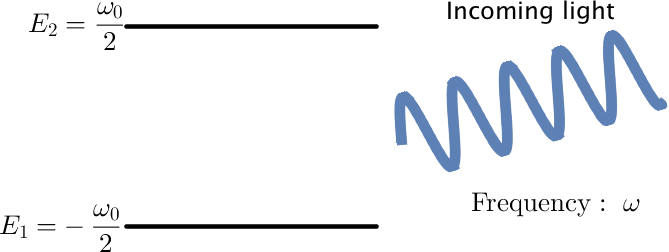
\includegraphics[width=0.6\textwidth]{chapters/assets/app/rabi-diagram.png}
    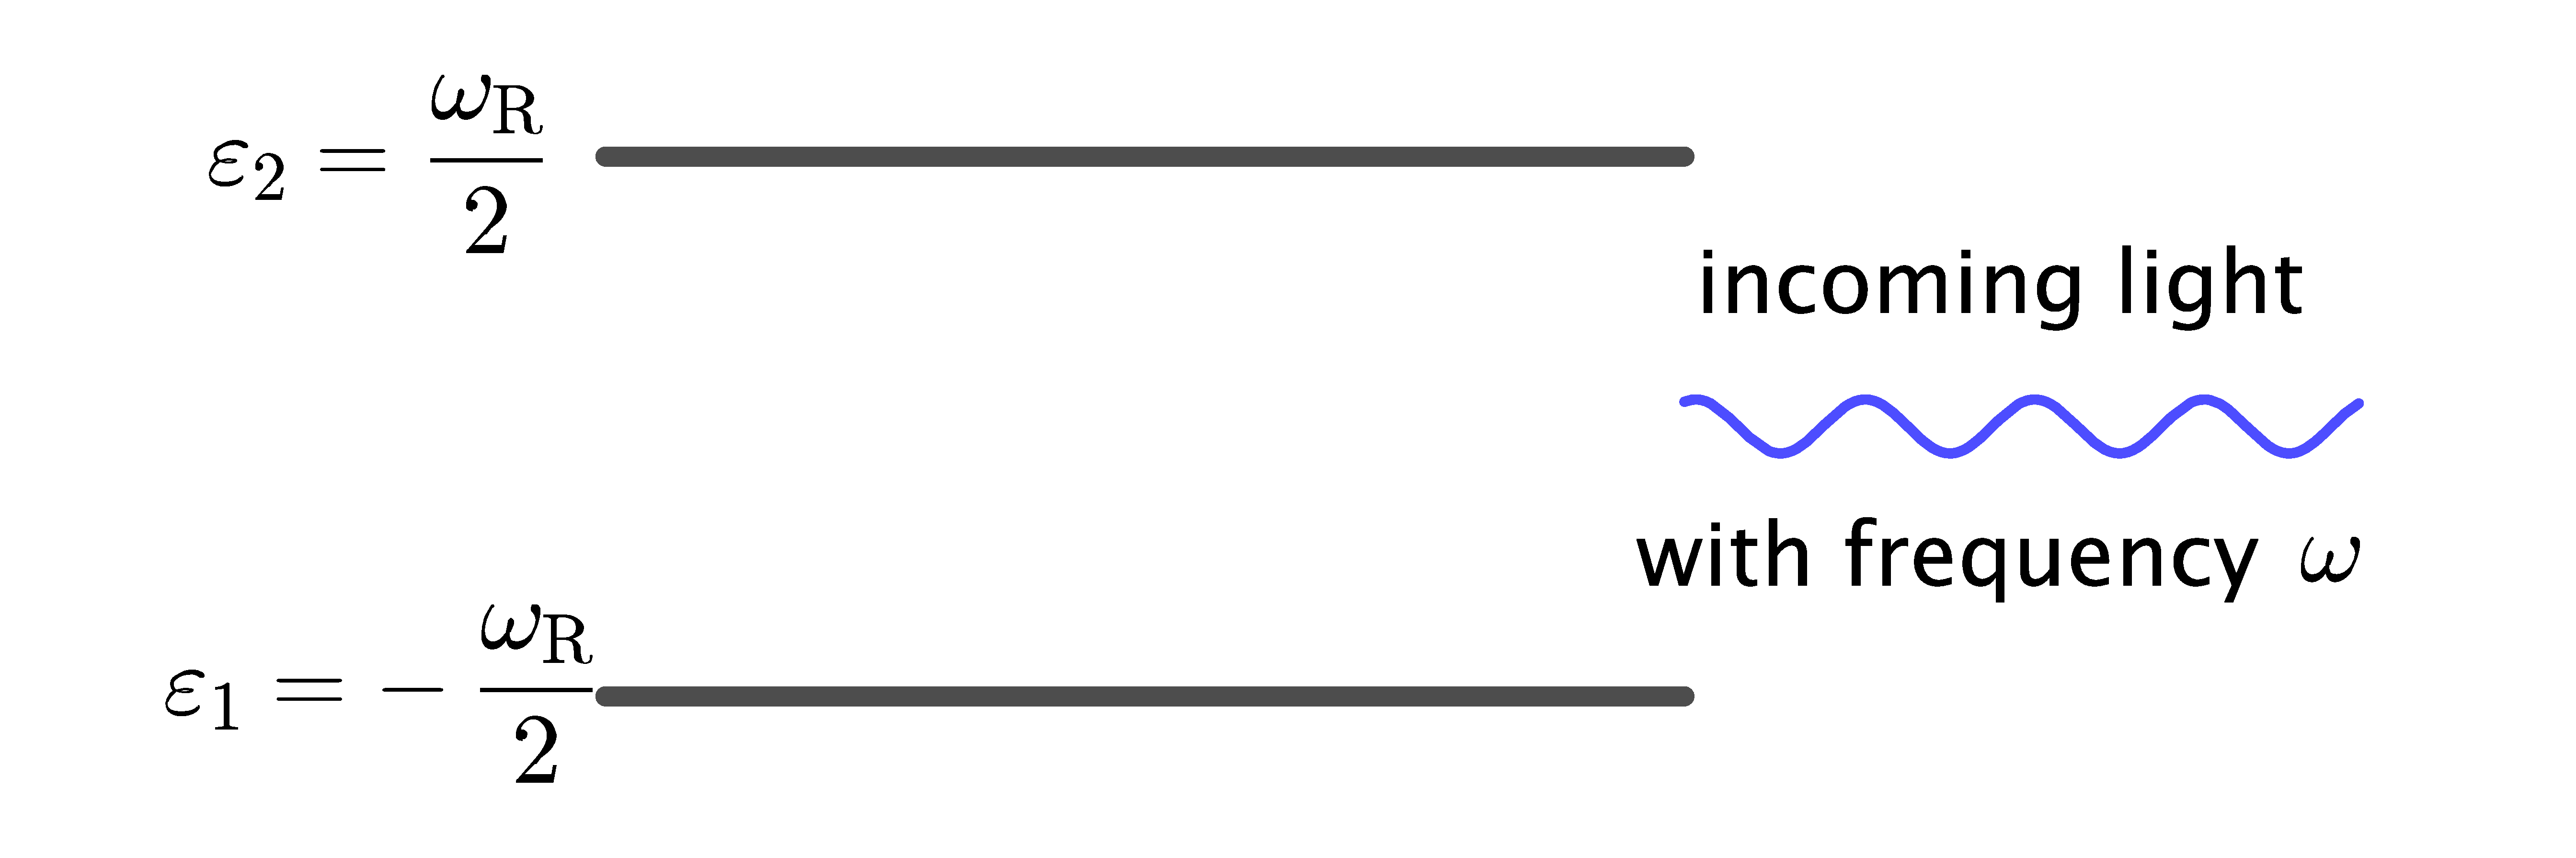
\includegraphics[width=0.7\textwidth]{chapters/assets/matter/rabi-illustrative-diagram}
    \caption{A two-level quantum system that experiences the Rabi oscillation. The resonance happens when the frequency of the driving field $\omega$ equals the energy gap $\omega_\RR = \epsilon_2 - \epsilon_1$.}
    \label{chap:app-sec:rabi-oscillations-fig:rabi-diagram}
\end{figure}

A two-level quantum system with energy gap $\delta\varepsilon = \omega_{\RR}$ can experience Rabi oscillations when light of frequency $\omega$ shines on it (see Fig.~\ref{chap:app-sec:rabi-oscillations-fig:rabi-diagram}).
The Hamiltonian for the system is
\begin{equation}
    \mathsf H_{\RR} = -\frac{\omega_{\RR}}{2}\sigma_3 - \frac{A_{\RR} }{2}  \left( \cos(k_{\RR} t +\phi_{\RR})\sigma_1  - \sin(k_{\RR} t +\phi_{\RR}) \sigma_2\right),
    \label{rabi-oscillation-single-perturbation}
\end{equation}
where $A_{\RR}$ and $k_{\mathrm{R}}$ are the amplitude and frequency of the driving field, respectively. The Hamiltonian $\mathsf H_\RR$ can be mapped into a vector using the flavor isospin picture:
\begin{equation*}
% H_{\mathrm R}
% = - \frac{\boldsymbol{\sigma}}{2} \cdot (\mathbf{H}_3 + \mathbf{H}_+ ) ,
\vec H_{\RR} = \vec H_3 + \vec H_+,
\label{chap:matter-eqn:rabi-hamiltonian-h3-hplus}
\end{equation*}
where
\begin{equation}
    \vec{H}_3 =  \begin{pmatrix}
    0 \\ 0 \\ \omega_{\mathrm R}
    \end{pmatrix} \quad \text{and} \quad
    \vec{H}_+ =  \begin{pmatrix}
    A_{\mathrm{R}} \cos(k_{\mathrm{R}} t +\phi_{\mathrm{R}}) \\
    - A_{\mathrm{R}} \sin(k_{\mathrm{R}} t +\phi_{\mathrm{R}}) \\
    0
    \end{pmatrix}.
    \label{chap:app-sec:rabi-eqn:h3-and-hplus}
\end{equation}
The vector $\vec{H}_3$ is the vector aligned with the third axis and $\vec{H}_+$ is a vector rotating in a plane perpendicular to $\vec{H}_3$ (see Fig.~\ref{chap:app-sec:rabi-fig:rabi-static-frame}). The wave function $\Psi=(\psi_1,\psi_2)^{\mathrm{T}}$ is also used to define the state vector $\vec{s}$
\begin{equation}
    \vec{s} = \Psi^\dagger \frac{\vec{\sigma}}{2}\Psi
    = \frac{1}{2}\begin{pmatrix}
    2\,\mathrm{Re}\,(\psi_1^* \psi_2) \\
    2\,\mathrm{Im}\,(\psi_1^*\psi_2) \\
    \lvert \psi_1 \rvert^2 - \lvert \psi_2 \rvert^2
    \end{pmatrix}
\end{equation}



\begin{figure}[htbp]
	\centering
	\begin{subfigure}[t]{0.5\textwidth}
		\centering
		\includegraphics[width=0.8\textwidth]{chapters/assets/matter/rabi-isospin-static-frame}
		\caption{Static frame}\label{chap:app-sec:rabi-fig:rabi-static-frame}
	\end{subfigure}%
	% \quad
	\begin{subfigure}[t]{0.5\textwidth}
		\centering
		\includegraphics[width=0.85\textwidth]{chapters/assets/matter/rabi-isospin-rotating-frame}
		\caption{Corotating frame}\label{chap:app-sec:rabi-fig:rabi-rotating-frame}
	\end{subfigure}
	\caption{
  Rabi oscillations in different frames. The vectors $\vec H_3$ and $\vec H_+$ are defined in Eqn.~\ref{chap:app-sec:rabi-eqn:h3-and-hplus}. The red dashed vector $\vec s$ represents the quantum state of the system, and the black solid vectors are for the Hamiltonians in the corresponding frames.
  }\label{chap:app-sec:rabi-fig:rabi-frames}
\end{figure}


The third component of $\vec{s}$, which is denoted as $s_3$, is within range $[-1/2,1/2]$. The two limits, $s_3=-1/2$ and $s_3=1/2$ stand for the two-level system in the high energy state and the low energy state, respectively. If the two-level system has equal probabilities to be in the high energy state and the low energy state, one has $s_3=0$. The equation of motion is a precession equation similar to Eqn.~\ref{chap:basics-sec:flavor-isospin-pic-eqn:eom-precession}. In this example, the total ``Hamiltonian vector" $\vec H_\RR$ is not static since it has a rotating component $\vec H_+$. I need a better frame to understand the evolution of the state vector $\vec s$.

% \begin{figure}[htbp]
%         \centering
%         \includegraphics[width=\columnwidth, trim={20cm 10cm 50cm 10cm},clip]{chapters/assets/rabi/rabi-isospin-rotating-frame}
%     \caption{Rabi oscillations in corotating frame. The red dashed vector is the flavor isospin, while the black solid vectors are the vectors of Hamiltonian. The flavor isospin vector is precessing around vector of total Hamiltonian $\vec{H}_3+\vec{H}_+$.}
%     \label{fig-rabi-isospin-rotating-frame}
% \end{figure}



A more convenient frame is the one that corotates with $\vec{H}_+$, which is depicted in Fig.~\ref{chap:app-sec:rabi-fig:rabi-rotating-frame}. The equation of motion in this frame is
\begin{equation}
\frac{\mathrm d}{\mathrm d t } \vec{s} = \vec{s} \times (\vec{H}'_3 + \vec{H}_+),
\end{equation}
where
\begin{equation}
\vec{H}'_3 = \begin{pmatrix}
    0 \\ 0 \\  \omega_{\mathrm{R}} - k_{\mathrm R}
  \end{pmatrix}, \quad \text{and} \quad \vec{H}'_+ = \begin{pmatrix}
    A_{\mathrm{R}} \\ 0 \\  0
    \end{pmatrix}.
\end{equation}
The state vector $\vec{s}$ precesses around the static vector $\vec{H}'_3 + \vec{H}'_+$ in this corotating frame with a frequency
\begin{equation}
    \Omega_{\mathrm R} = \sqrt{ \lvert A_{\mathrm{R}}\rvert^2 + (k_{\mathrm{R}} - \omega_{\mathrm R})^2 },
    \label{app:rabi-frequency}
\end{equation}
which is known as the Rabi frequency.
Projecting the state vector $\vec{s}$ on to the third axis, I obtain
\begin{equation}
s_3 = \frac{1}{2} - \frac{\lvert A_{\mathrm R}\rvert ^2}{\Omega_{\mathrm R}^2}\sin^2\left(\frac{\Omega_{\mathrm R}}{2} t\right).
\end{equation}
Such a system has an analytical transition probability from the low energy state to the high energy state, known as the Rabi formula,
\begin{equation}
    P(t) = \frac{1}{2}(1- 2 s_3(t))= \frac{1}{ 1 + \RD^2 } \sin^2 \left( \frac{\Omega_{\mathrm R}}{2} t \right),
    \label{app:rabi-system-transition-probability}
\end{equation}
where 
\begin{equation}
    \RD = \left\lvert \frac{ k_{\mathrm R} - \omega_{\mathrm R}}{A_{\mathrm R}} \right\rvert.
    \label{chap:app-sec:rabi-oscillations-eqn:relative-detuning-def}
\end{equation}
is the relative detuning.

%Similar to the neutrino oscillations in a uniform matter profile (see Eqn.~\ref{chap:basics-sec:flavor-isospin-pic-fig:msw-adiabatic-critical}), 
The resonance of Rabi oscillations occurs when $\vec{H}'_3=0$ in the corotating frame and $\vec{s}$ oscillates between $+1/2$ (the low energy state) and $-1/2$ (the high energy state). The transition amplitude is determined by relative detuning $\RD$ as illustrated by two numerical examples in Fig.~\ref{app-fig:rabi-examples}. The resonance width is determined by the amplitude of the driving field $A_\RR$ as shown in Fig.~\ref{app-fig:rabi-resonance-width}.
% The detuning, which is defined by $k_{\mathrm{R}} - \omega_{\mathrm R}$, determines how off resonance the system is, and 
% The amplitude of the driving field $A_{\mathrm{R}}$ determines the resonance width,
% \begin{align}
% \text{Detuning} =&~\lvert k_{\mathrm{R}} - \omega_{\mathrm R} \rvert, \\
% \text{Resonance Width} =&~\lvert A_{\mathrm R} \rvert.
% \end{align}
% as shown in Fig.~\ref{app-fig:rabi-resonance-width}.
% The amplitude $A_\RR$ is the dominant factor of oscillation frequency when the system is close to resonance. The phase $\phi_{\mathrm{R}}$ of the driving potential in Eqn.~\ref{rabi-oscillation-single-perturbation} has no effect on the transition probability since it only determines the initial phase of driving Hamiltonian vector $\vec{H}_+$. Fig.~\ref{app-fig:rabi-examples} shows two examples of Rabi oscillations.

\begin{figure}[htbp]
    \centering
    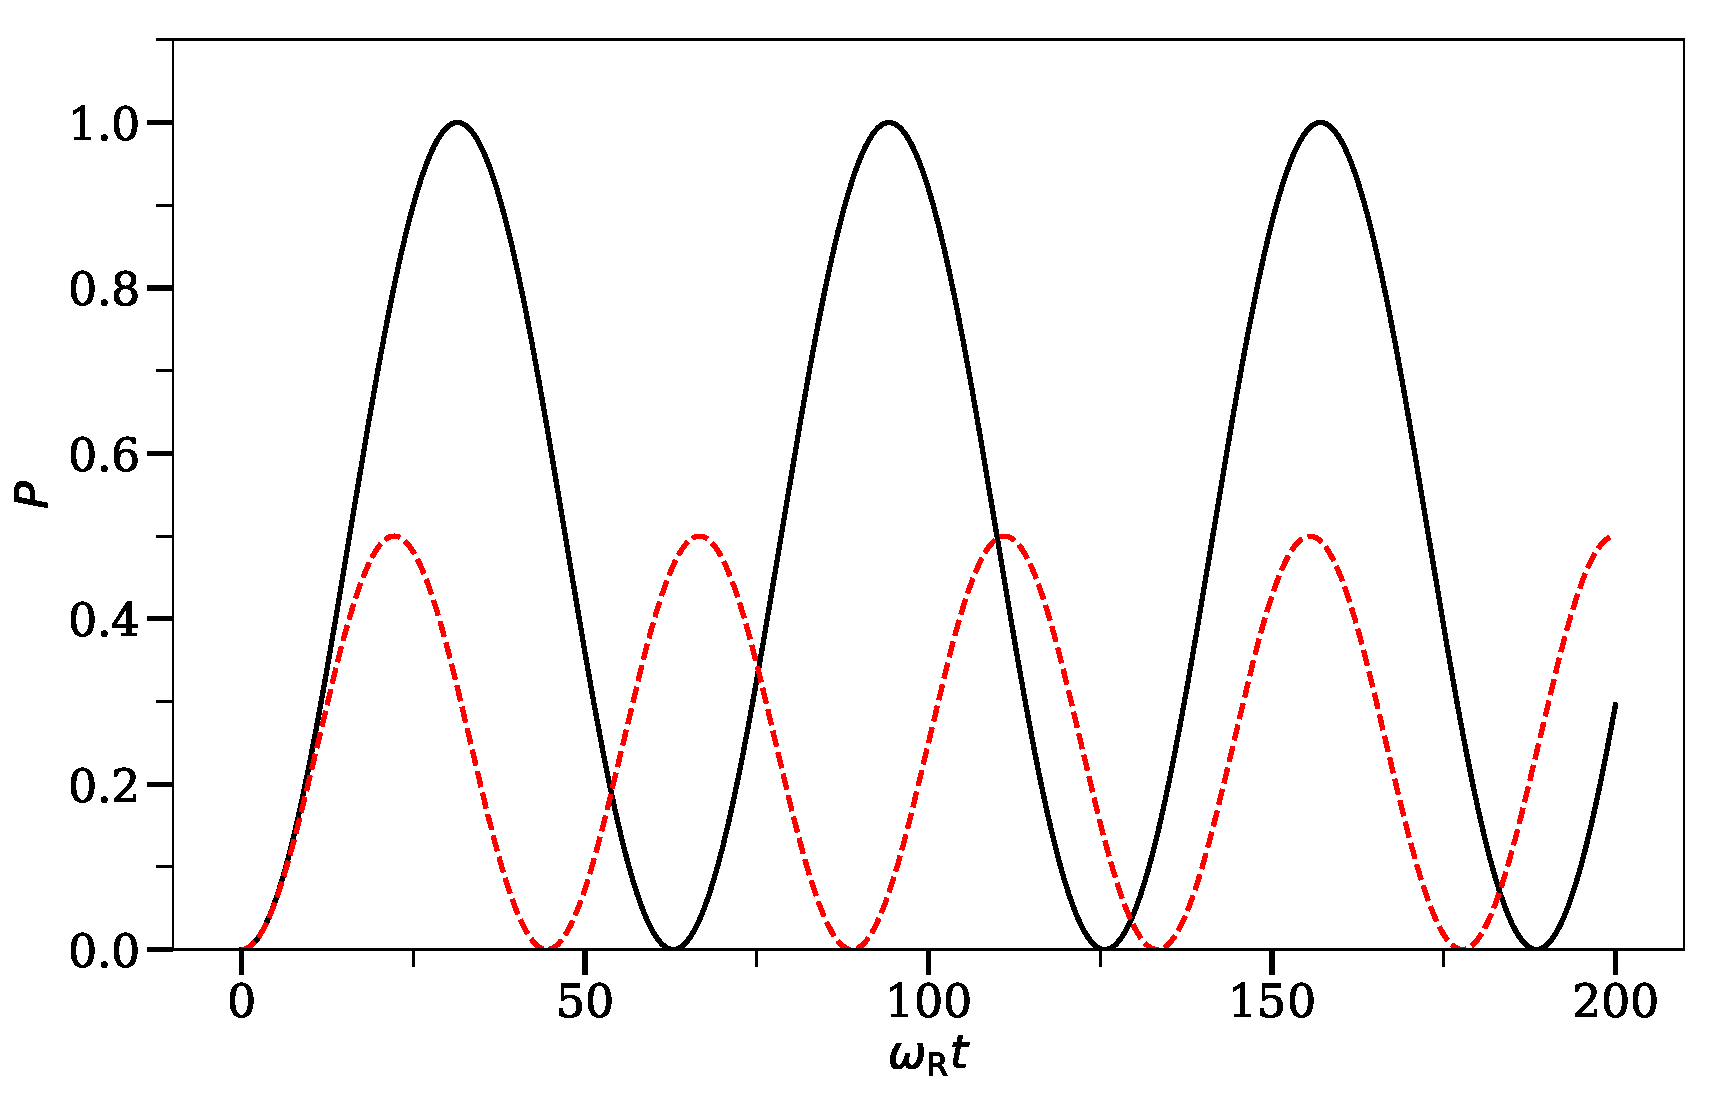
\includegraphics[width=\textwidth]{chapters/assets/app/rabi-oscillations}
    \caption{The transition probabilities $P$ between the energy states of a two-level quantum system when external driving fields with frequencies $k_\RR = \omega_\RR$ and $k_\RR=1.1\omega_\RR$ are applied, respectively. The corresponding relative detunings are $\RD = 0$ and $\RD = 1$, respectively. The amplitudes of the driving fields are $A_\RR=0.1\omega_\RR$ in both cases. }
    \label{app-fig:rabi-examples}
\end{figure}



\begin{figure}[htbp]
    \centering
    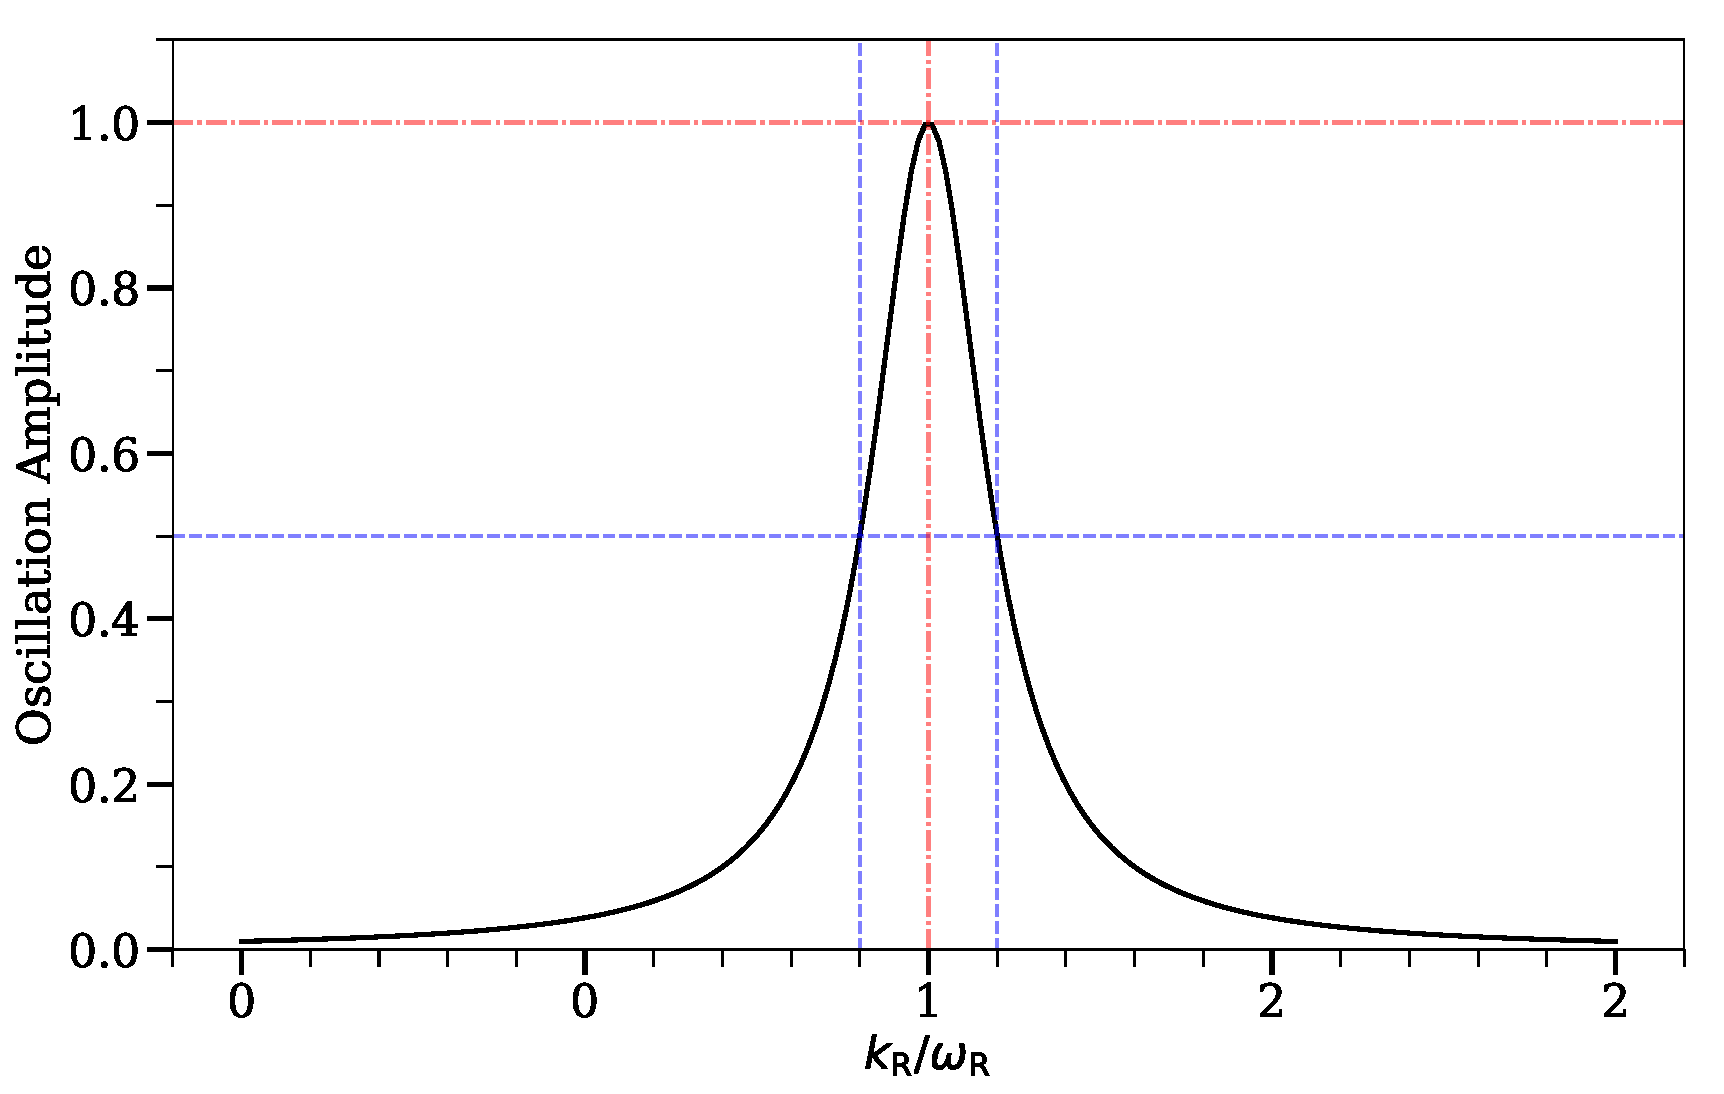
\includegraphics[width=\textwidth]{chapters/assets/app/rabi-resonance-width}
    \caption{The amplitude of Rabi oscillations as a function of the frequency of the external driving field $k_\RR$. The maximum amplitude occurs at $k_\RR/\omega_\RR=1$. The resonance width is defined to be the difference of $k_\RR$ at which the amplitudes are 1/2.}
    \label{app-fig:rabi-resonance-width}
\end{figure}

% \subsection{Interference Between the Driving Fields}

In many cases, the two-level quantum system has more than one driving fields. I will refer to each of the driving field as a Rabi mode. Here I consider the Hamiltonian with two Rabi modes:
\begin{align}
    \mathsf H_{\mathrm R} =& -\frac{\omega_{\mathrm R}}{2}\sigma_3 - \frac{A_{1} }{2}  \left( \cos(k_{1} t +\phi_{1})\sigma_1  - \sin(k_{1} t +\phi_{1}) \sigma_2\right) \nonumber\\
    & - \frac{A_{2} }{2}  \left( \cos(k_{2} t +\phi_{2})\sigma_1  - \sin(k_{2} t +\phi_{2}) \sigma_2\right).
    \label{chap:matter-sec:single-frequency-eqn:hamiltonian-two-level}
\end{align}
I decompose it into $\vec{H}_{\mathrm R}=\vec{H}_3 + \vec{H}_{1} + \vec{H}_2$, where
\begin{equation*}
    \vec{H}_1 =  \begin{pmatrix}
     A_{1} \cos(k_{1}t+\phi_{1}) \\
     -A_{1} \sin(k_{1}t+\phi_{1})  \\
     0
   \end{pmatrix} \quad\text{and}\quad   \vec{H}_2 =  \begin{pmatrix}
     A_{2} \cos(k_{2}t+\phi_{2}) \\
     -A_{2} \sin(k_{2}t+\phi_{2})  \\
     0
      \end{pmatrix}.
\end{equation*}
I will assume that the first Rabi mode $\vec{H}_1$ is almost on resonance, and the second one $\vec H_2$ is off resonance, i.e.,% $\vec H_1$ and $\vec H_2$ are two rotating vectors as a function of $r$ with frequencies $k_1$ and $k_2$ in this vector space, while $\vec H_3$ is perpendicular to $\vec H_1$ and $\vec H_2$.
%The most general condition that we can drop the new perturbation $\vec{H}_2$ is to make sure $k_2$ is far from the resonance condition compared to the resonance width,
\begin{equation}
\RD_1 \lesssim 1 \quad \text{and} \quad
\RD_2 \gg 1,
\end{equation}
where
\begin{equation}
\RD_i\equiv \frac{\lvert k_i -\omega_{\mathrm R}\rvert}{\lvert A_i\rvert}
\end{equation}
is the relative detuning of the $i$th Rabi mode.

% In fact, I will derive a more stringent criteria for the significance of the second driving potential.
% The transition amplitude between the two states becomes
% \begin{equation}
% P(t) = \frac{1}{1+\RD^2}\sin^2\left(\frac{\Omega_{\mathrm{R}}}{2}t\right).
% \end{equation}
% \begin{figure}[htbp]
%     \centering
%     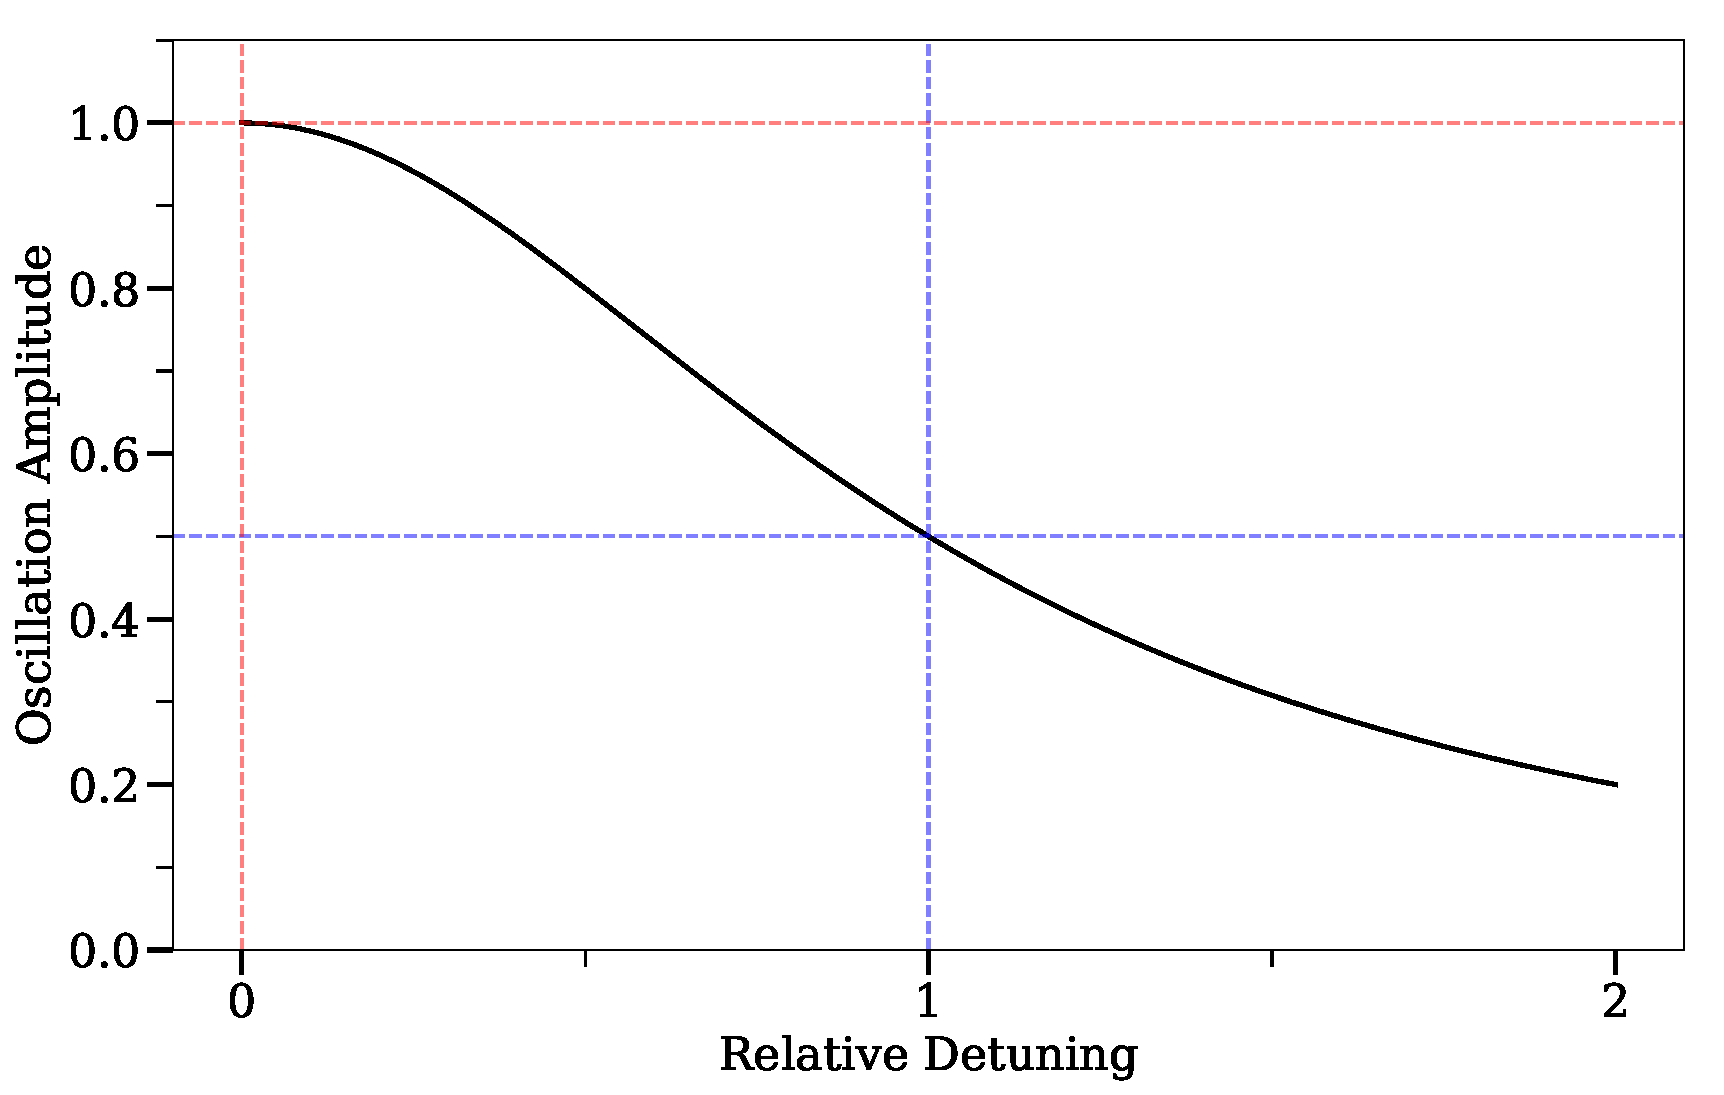
\includegraphics[width=\textwidth]{chapters/assets/app/rabi-resonance-detuning}
%     \caption{Rabi oscillations for two different relative detunings $\RD$. $\RD=1$ is the resonance condition. The amplitude reach maximum when $\RD=0$, i.e., $k_\RR=\omega_\RR$. }
%     \label{app-fig:rabi-resonance-width}
% \end{figure}
%Suppose I have a Rabi oscillation system with two modes, one of which is at resonance with frequency $k_1=\omega_{\mathrm m}$ and the other mode with frequency $k_2$ that is off resonance. In some cases, there can be a significant transition amplitude decrease because of the off resonance frequency $k_2$, which can be interpreted as shift of energy gap due to the frequency $k_2$.
% To model the effect, I construct a Rabi oscillation Hamiltonian with two modes of different frequency,
% \begin{equation}
% \mathsf H^{(\mathrm{m})}  = -\frac{\omega_{\mathrm{m}}}{2} \sigma_3 - \frac{1}{2} \sum_{n=1}^N  A_n \cos (k_n r) \sigma_1 + \frac{1}{2} \sum_{n=1}^N  A_n \sin (k_n r) \sigma_2,
% \label{eq-hamiltonian-rabi-two-modes-interference}
% \end{equation}
% where $N=2$ for two frequency case. To show the destruction effect, the Hamiltonian Eqn.~\ref{eq-hamiltonian-rabi-two-modes-interference} is reformulated into a vector in flavor-isospin space,
% \begin{equation}
% \mathbf H = \mathbf H_3 + \mathbf H_1 +\mathbf H_2 = \begin{pmatrix}
% 0\\
% 0\\
% \omega_\mm
% \end{pmatrix} + \begin{pmatrix}
% A_1 \cos (k_1 r)\\
% -A_1 \sin (k_1 r)\\
% 0
% \end{pmatrix} + \begin{pmatrix}
% A_2 \cos (k_2 r)\\
% -A_2 \sin (k_2 r)\\
% 0
% \end{pmatrix}.
% \end{equation}
Although the second Rabi mode is off resonance, it can interfere with the Rabi oscillation caused by the first Rabi mode.
To see this effect, I will use the frame that corotates with $\vec H_2$. In the corotating frame, the two Rabi modes have frequencies $k_1'=k_1-k_2$ and $k_2'=0$, respectively, and $\vec H'_3 = ( 0,0, \omega_{\RR}- k_2 )^{\mathrm{T}}$. Obviously, the Hamiltonian vector in this corotating frame is similar to Eqn.~\ref{chap:matter-eqn:rabi-hamiltonian-h3-hplus} except with the replacements
\begin{equation}
    \vec H_3 \to \vec H'_3 + \vec H'_2  \quad \text{and} \quad \vec H_+ \to \vec H'_1.
\end{equation}
%The resonance mode $\vec H_1$ retains on the resonance condition since $k_1'=\omega_{\RR}'$, i.e. $k_1-k_2 = \omega_{\RR}-k_2$, holds in the new frame. On the other hand, we have two static fields $\vec H_3$ and $\vec H_2$ together as the new energy gap, as long as 
I will further assume that $\lvert A_2\rvert \ll \omega_\RR$ so that the new energy gap is
\begin{align}
    \tilde\omega_{\mathrm{R}}' &\equiv \lvert \vec H'_3 + \vec H'_2 \rvert \nonumber\\
    &= \sign (\omega_{\RR}- k_2 ) \sqrt{ (\omega_{\RR}- k_2 )^2 + A_2^2 } \nonumber\\
    &\approx \omega_{\mathrm R} - k_2 + \frac{1}{2}\frac{A_2^2}{\omega_{\mathrm R} - k_2},
    \label{eq-new-energy-gap-due-to-second-mode-approximation}
\end{align}
where I kept only up to the first order of the Taylor series. I can calculate the new relative detuning of the system to be
\begin{align}
    \RD' &= \frac{\lvert k_1' - \tilde \omega_{\mathrm R}' \rvert}{\lvert A_1 \rvert}\nonumber\\
    &\approx \left \lvert \frac{ k_1-\omega_{\mathrm R}}{ A_1} + \frac{ A_2^2 }{2  A_1 ( k_2 - \omega_{\mathrm R})} \right  \rvert.
    % &= \left \lvert  \frac{\sign({ k_1-\omega_{\mathrm R}})}{\sign (k_2 - \omega_{\mathrm R})} \RD_1 +  \frac{ A_2 }{2 A_1 \RD_2 }\right \rvert ,
    \label{app:chap:matter-eq:relative-detuning-changed}
\end{align}
% where $\RD_1$ and $\RD_2$ are the relative detuning of the first mode and second mode, respectively. They are defined as
% \begin{equation*}
% \RD_i =  \left\lvert \frac{ k_i - \omega_{\mathrm R}}{A_i} \right \rvert.
% \end{equation*}
One can adjust frequency of the off-resonance Rabi mode $k_2$ to decrease or increase $\RD$ so that the system is close to or further away from the resonance. The criterion for the off-resonance Rabi mode to have a significant impact on the Rabi resonance is
\begin{equation}
    \left\lvert  \frac{ A_2^2 }{2  A_1 ( k_2 - \omega_{\mathrm R})} \right\rvert \gtrsim 1 \quad \text{or} \quad \lvert A_2\rvert \gtrsim \sqrt{ 2 \lvert A_1 (k_2 - \omega_\RR) \rvert }
    \label{chap:matter-sec:single-frequency-eqn:criterion-for-a2}
\end{equation}
% In principle, the energy gap of the first frequency can be changed to approach the resonance or escape the resonance by carefully arranging the second frequency, which is also obvious from Eqn.~(\ref{chap:matter-eq:relative-detuning-changed}). For the purpose of the section we first discuss the most important destruction effect by choosing $\RD_1 = 0$. We observe the importance of the relative detuning. For the second mode to significantly interfere with the first mode, we need a small $\RD_2$ and a large amplitude or width $A_2\gg A_1$.




\section{\label{chap:matter-sec:background}Background Matter Basis}

% \fbox{TODO: Explain why two flavor} didn't add this because the three flavor is really very different.

% I will write down the equation of motion for neutrinos propagating through a general matter profile $\lambda(r)$ where $r$ is the trajectory of neutrinos. The Hamiltonian of neutrino oscillations is Eqn.~\ref{chap:basics-sec:msw-eqn:hamiltonian-matter-effect}. The dynamics of neutrino flavor conversion is determined by the Schr\"{o}dinger equation:
% \begin{equation*}
%     \mathrm i\frac{\mathrm d}{\mathrm d r}\Psi(r) = \frac{1}{2} \left(
%     (- \omega_{\mathrm{v}}\cos 2\theta_{\mathrm{v}} + \lambda(r) ) \sigma_3 + \omega_{\mathrm{v}}\sin 2\theta_{\mathrm{v}} \sigma_1
%     \right)
%     \Psi(r),
% \end{equation*}
% where $\Psi(r)$ is the wave function in flavor basis. For the two flavor scenario, the wave function is written as
% \begin{equation}
% 	 \Psi(r) = \begin{pmatrix}
%     \psi_{\ee} \\
%     \psi_{\xx}
% 	\end{pmatrix},
% \end{equation}
% where $\psi_{\ee}$ and $\psi_{\xx}$ are the amplitudes for electron flavor and the other flavor ($\mu$ flavor or $\tau$ flavor) respectively.

For a uniform matter density $\lambda(r) = \lambda_0$, one can define a matter basis in which the Hamiltonian is diagonalized:
\begin{equation}
\mathsf H^{(\mm)}  = \mathsf U^\dagger \mathsf H^{(\ff)} \mathsf U = -\frac{\omega_\mm}{2} \sigma_3,
\end{equation}
where
\begin{equation}
\mathsf U = \begin{pmatrix}
\cos \theta_\mm & \sin \theta_\mm \\
\sin\theta_\mm & \cos \theta_\mm
\end{pmatrix}
\end{equation}
with
\begin{equation*}
\theta_{\mathrm{m}}= \frac{1}{2} \arctan\left(
\frac{\sin 2\theta_{\mathrm v}}{ \cos 2\theta_{\mathrm v} - \lambda_0/\omega_{\mathrm v} } \right),
\label{chap:matter-sec:background-eqn:thetam}
\end{equation*}
and
\begin{equation}
\omega_{\mathrm{m}} = \omega_{\mathrm{v}} \sqrt{ ( \lambda_0/\omega_{\mathrm{v}} - \cos (2\theta_{\mathrm{v}}) )^2 + \sin^2(2\theta_{\mathrm{v}}) }
\label{chap:matter-sec:background-eqn:omegam}
\end{equation}
is the neutrino oscillation frequency in matter.

In the rest of the chapter, I will consider profiles of the form
\begin{equation}
    \lambda(r) = \lambda_0 + \delta \lambda(r),
    \label{eq-general-matter-profile}
\end{equation}
where $\delta \lambda(r)$ describes the fluctuation of the matter density. I will use the background matter basis defined in Eqn.~\ref{chap:matter-sec:background-eqn:thetam} and Eqn.~\ref{chap:matter-sec:background-eqn:omegam}. In this basis, the Hamiltonian reads
\begin{equation}
    \mathsf H^{(\mathrm{m})} = -\frac{\omega_\mm}{2} \sigma_3 + \frac{1}{2} \delta\lambda(r) \cos 2\theta_{\mathrm m} \sigma_3
     - \frac{1}{2} \delta\lambda(r) \sin 2\theta_{\mathrm m} \sigma_1.
    \label{eq-hamiltonian-bg-matter-basis-general}
\end{equation}

In this chapter, I will focus on the transition probability between the background matter eigenstates
\begin{equation}
    \begin{pmatrix}
        \ket{\nu_{\mathrm L}} \\
        \ket{\nu_{\mathrm H}}
    \end{pmatrix} = \mathsf U^\dagger \begin{pmatrix}
        \ket{\nu_{\mathrm e}} \\
        \ket{\nu_{\mathrm x}}
    \end{pmatrix}.
\end{equation}
Given this transition probability, it is trivial to calculate the flavor conversion.

All the numerical examples in this chapter are calculated with $\sin^2(2\theta_{\mathrm v}) = 0.093$ and $\omega_{\vv} = 3.75\times 10^{-17}\mathrm{MeV}^2$.
%$\delta m^2 = 2.6\times 10^{-3}\mathrm{eV}^2$.



%%%%%%%%%%%%%%%%%%%%%%%%%%%%%%%%%%%%%%%%%%%%%%%%%%%%
%% Single frequency
%%%%%%%%%%%%%%%%%%%%%%%%%%%%%%%%%%%%%%%%%%%%%%%%%%%%



\section{\label{chap:matter-sec:single}Single-Frequency Matter Profile}%


% In this section I will present a simple picture to explain neutrino parametric resonance in matter by utilizing the theory of Rabi oscillations. Rabi oscillations have been well studied in quantum optics~\cite{Boyd2008}. It describes the transition between different quantum states due to an oscillatory external driving field, where maximum transition or resonance happens when the frequency of the external driving field equals the energy gap between two quantum states. In this section, I will first derive the Rabi oscillation transition probabilities using the neutrino flavor isospin method introduced in Ref.~\cite{Duan2006a}. Then I will apply the results of Rabi oscillations to the neutrino oscillation with a single frequency matter profile.




% chap:matter-sec:single-frequency-matter-profile
%%%%%%%%%%%%%%%%%%%%%%%%%%%%%%%%%%%%
%%%%%%%%% Rabi oscillation
%%%%%%%%%%%%%%%%%%%%%%%%%%%%%%%%%%%%
% \subsection{\label{chap:matter-sec:single-frequency-matter-profile}Single-Frequency Matter Profile}


I will examine the neutrino flavor conversion in a single-frequency matter profile $\delta\lambda(r) = \lambda_1 \cos(k_1 r)$. I will assume that the perturbation is small so that $\lambda_1 \ll \omega_\mm$. The Hamiltonian in the background matter basis becomes
\begin{equation}
\mathsf H^{(\mm)} = - \frac{\omega_\mm}{2}\sigma_3  + \frac{1}{2} \lambda_1 \cos(k_1 r) \cos 2\theta_\mm \sigma_3 - \frac{1}{2} \lambda_1 \cos(k_1 r)\sin 2\theta_\mm \sigma_1.
\label{chap:matter-sec:single-fequency-eq:hamiltonian-bg-matter-basis-single-frequency}
\end{equation}
I will consider the case when $k_1$ is not far away from resonance, i.e., $k_1 \sim \omega_\mm$. As will be proven later, the oscillating $\sigma_3$ term $\frac{1}{2} \lambda_1 \cos(k_1 r) \cos 2\theta_\mm \sigma_3$ in the above Hamiltonian has little effect on the transition probabilities in this case. With the oscillating $\sigma_3$ term removed, 
\begin{align}
    \mathsf H^{(\mm)} &\to -\frac{\omega_{\mathrm m}}{2} \sigma_3  - \frac{1}{2} A_1 \cos ( k_1 r)  \sigma_1 + \frac{1}{2} A_1\sin(k_1 r) \sigma_2 \nonumber\\
    &\phantom{\to} - \frac{1}{2} A_2 \cos ( k_2 r)  \sigma_1 + \frac{1}{2} A_2\sin(k_2 r) \sigma_2  
    \label{eq-hamiltonian-bg-matter-basis-single-frequency}
\end{align}
where
\begin{align}
    A_1 = A_2 = \frac{\lambda_1 \sin(2\theta_\mm) }{2} \quad \text{and} \quad k_2 = -k_1.
    \label{chap:matter-sec:single-eqn:rabi-amplitudes}
\end{align}
This is the same as the Hamiltonian $\mathsf H_{(\RR)}$ in Eqn.~\ref{chap:matter-sec:single-frequency-eqn:hamiltonian-two-level}.
Because the second Rabi mode is off resonance and its amplitude is too small to satisfy the criterion in Eqn.~\ref{chap:matter-sec:single-frequency-eqn:criterion-for-a2}, it can be neglected and Rabi formula in Eqn.~\ref{app:rabi-system-transition-probability} can be applied with $A_\RR=A_1$, $k_\RR=k_1$, and $\omega_\RR = \omega_\mm$.
% The external driving field frequency is $\pm k_1$ and the energy gap is $\omega_{\mathrm m}$. I can decompose $\cos( k_1 r )$ into two exponential functions so that we have two Rabi modes $k_1$ and $-k_1$. By neglecting the off-resonance frequency $-k_1$, the Hamiltonian can be simplified to
% \begin{align}
% \mathsf H^{(\mathrm{m})} \to & -\frac{\omega_{\mathrm m}}{2} \sigma_3  - \frac{1}{2} \lambda_1 \sin 2\theta_{\mathrm m} \cos( k_1 r ) \sigma_1\label{eq-hamiltonian-bg-matter-basis-single-frequency} \\
% \to & -\frac{\omega_{\mathrm m}}{2} \sigma_3  - \frac{1}{2} A_1 \exp (\mathrm ik_1 r) \sigma_1 \nonumber \\
% = & -\frac{\omega_{\mathrm m}}{2} \sigma_3  - \frac{1}{2} A_1 \cos ( k_1 r)  \sigma_1 + \frac{1}{2} A_1\sin(k_1 r) \sigma_2,\nonumber
% \label{chap:matter-sec:single-frequency-matter-profile-eqn:single-frequency-hamiltonian-approximation}
% \end{align}
% where I have used
% \begin{equation}
% A_1 = \frac{\lambda_1 \sin 2\theta_{\mathrm m} }{2}.
% \label{eq-define-a1}
% \end{equation}

% Now I have reduced the neutrino oscillations to Rabi oscillations. The resonance happens when the energy gap $\omega_{\mathrm m}$ is close to the external driving field frequency $k_1$, i.e., $\omega_{\mathrm m} \sim k_1$. As long as the resonance condition is satisfied, the transition probability between the two mass states should be predicted well using Rabi formula.
%To show that this conjecture of simplifying neutrino flavor conversions to Rabi oscillations is correct, 

I calculated the transition probability using the Hamiltonian in Eqn.~\ref{chap:matter-sec:single-fequency-eq:hamiltonian-bg-matter-basis-single-frequency} with $k_1/\omega_\mm=1$ and plotted it as black square markers in Fig.~\ref{fig-rabiOscillationsNeutrinoCoincidence}. As comparison I also plotted the transition probability obtained from the Rabi formula in Eqn.~\ref{app:rabi-system-transition-probability} as the dot-dashed curve in the same figure, which agrees with the numerical result very well. In this case, the first Rabi mode is exactly on resonance with relative detuning $\RD_1=0$. I calculated the transition probabilities for additional two cases with $k_1/\omega_\mathrm{m}=1-2\times 10^{-5}$ and $1-10^{-4}$, which have relative detunings $\RD_1 = 1$ and $5.2$, respectively. The Rabi resonance is suppressed as $\RD_1$ increases. The results obtained using the full Hamiltonian and those from the Rabi formula again agree very well. 

\begin{figure}[h!tbp]
                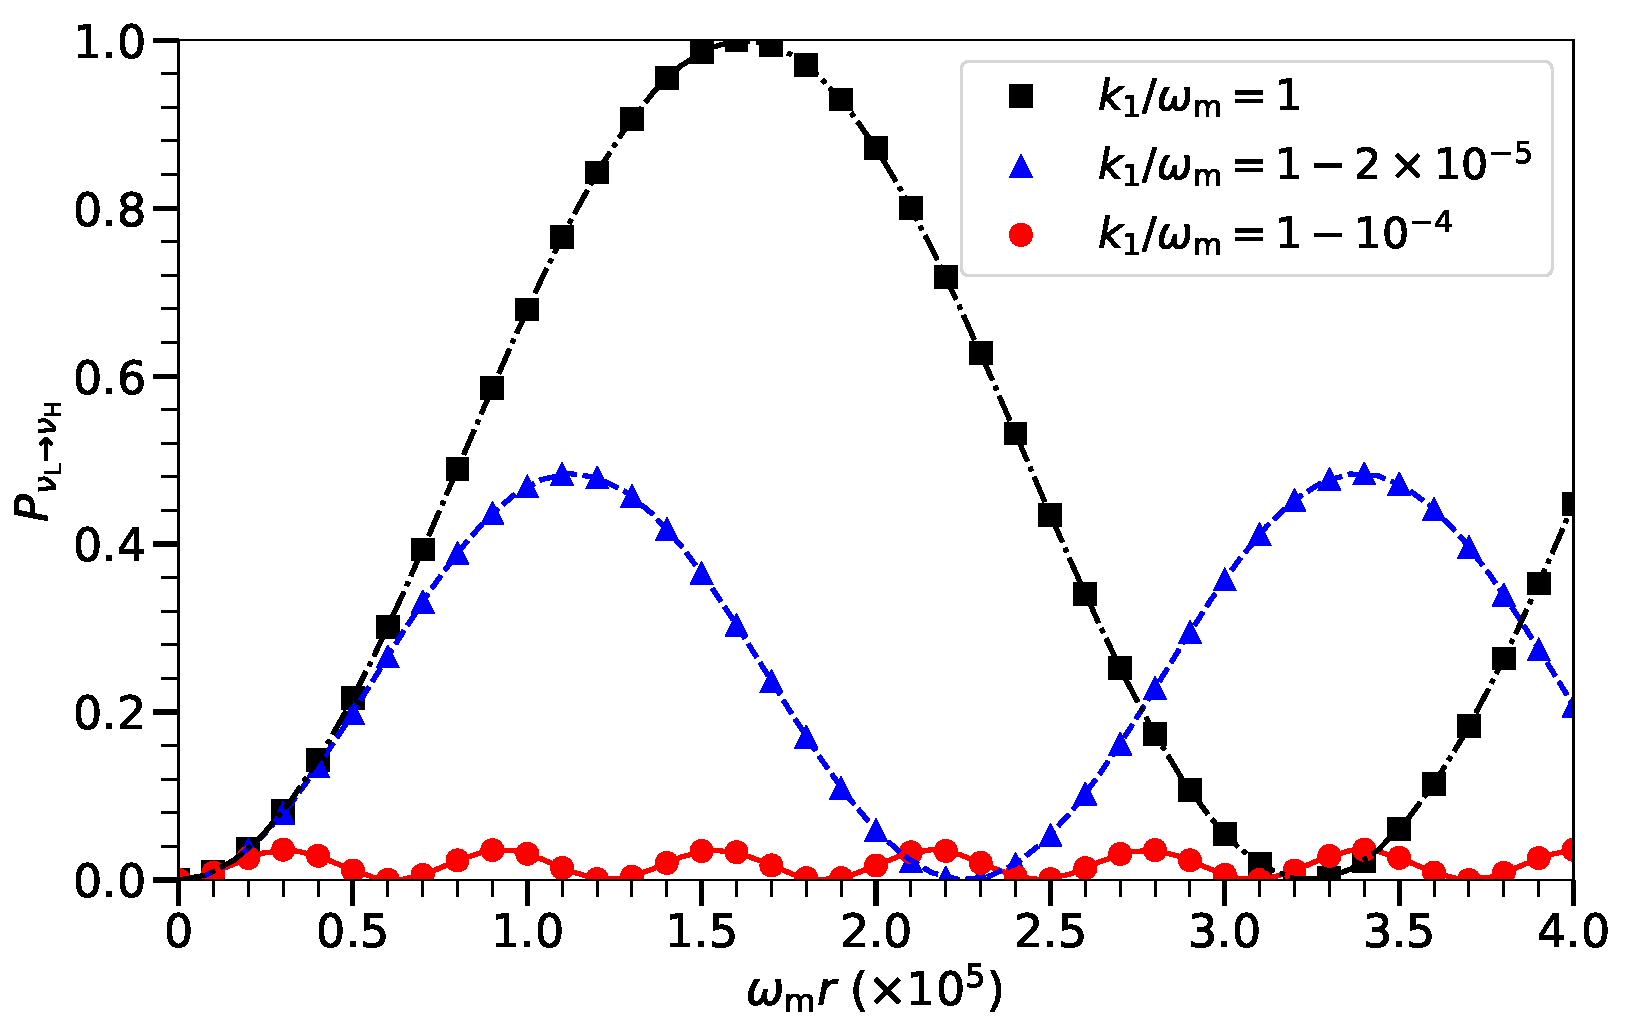
\includegraphics[width=\columnwidth]{chapters/assets/rabi/rabiOscillationsNeutrinoCoincidence-single-frequency}
                %rabiOscillationsNeutrinoCoincidence}
                \caption{The transition probabilities $P_{\nu_\mathrm{L}\to\nu_\mathrm{H}}$ as functions of distance $r$ for a neutrino propagating through matter profiles $\lambda(r)=\lambda_0 + \lambda_1 \cos (k_1 r)$ with different values of $k_1$ as labeled. The markers are for the numerical results obtained by using the Hamiltonian in Eqn.~\ref{chap:matter-sec:single-fequency-eq:hamiltonian-bg-matter-basis-single-frequency}, and the continuous curves are obtained using the Rabi formula in Eqn.~\ref{app:rabi-system-transition-probability}. In all three cases, $\lambda_0$ is half of the MSW resonance potential, and $\lambda_1/\omega_\mm=5.2\times 10^{-4}$.}
                \label{fig-rabiOscillationsNeutrinoCoincidence}
\end{figure}

% In Fig.~\ref{fig-rabiOscillationsNeutrinoCoincidence}, I have plotted the numerical results using markers as well as the prediction using Rabi formula using lines. The agreement between numerical solutions of neutrino transitions between mass states and Rabi formula will be explained more precisely in Sec.~\ref{sec:jacobi}. For now, we address the significance of relative detuning $\RD = \lvert k_1 - \omega_{\mathrm m} \rvert /\lvert A_1 \rvert$,  which is rigorously defined in Eqn.~\ref{chap:app-sec:rabi-oscillations-eqn:relative-detuning-def}. $\RD\to 0$ indicates that the neutrino oscillation is very close to resonance, while $\RD\to \infty$ indicates that the neutrino oscillation is far away from resonance. The corresponding relative detunings in Fig.~\ref{fig-rabiOscillationsNeutrinoCoincidence} are $0$, $1.0$, and $5.2$ for $k_1=\omega_{\mathrm{m}}$, $k_1=(1-2\times 10^{-5})\omega_{\mathrm m}$, and $k_1=(1-10^{-4})\omega_{\mathrm m}$.

% 0, 0.516197,1.03239,5.16197

For a single-frequency perturbation in the matter profile $\lambda(r) =\lambda_0 +  \lambda_1\sin(k_1 r)$, P. Krastev and A. Smirnov concluded that the parametric resonance condition is $\omega_{\mathrm{m}} \sim n k_1$, if
\begin{equation}
    \omega_{\mathrm{m,inst}}(r) = \omega_{\mathrm{v}} \sqrt{ ( \lambda(r)/\omega_{\mathrm{v}} - \cos (2\theta_{\mathrm{v}}) )^2 + \sin^2(2\theta_{\mathrm{v}}) }
\end{equation}
varies slowly with $r$~\cite{Krastev1989}. This condition is exactly the Rabi resonance condition when $n=1$. Higher order effects will be explained in Sec.~\ref{chap:matter-sec:single-revisted}.





\section{\label{chap:matter-sec:multiple-matter-frequencies}Multi-Frequency Matter Profiles}


The approach applied to the neutrino flavor transformation with a single-frequency matter profile can also be used in more general cases with multi-frequency matter profiles. Even though there is only one Rabi mode that is on resonance, the presence of many off-resonance Rabi modes may interfere with the on-resonance mode and suppress or enhance the neutrino flavor conversion. 

I will consider a matter profile with two Fourier modes:
\begin{equation}
    \lambda(r) = \lambda_0 + \lambda_1 \cos (k_1 r) + \lambda_2 \cos (k_2 r).
\end{equation}
%However, multi-frequency matter profile leads to multiple modes of Rabi oscillations, even with our simplified approach by dropping the oscillating $\sigma_3$ term in Hamiltonian. In this section, I will examine the neutrino oscillations in multi-frequency matter profiles using the interference effects discussed in Sec.~\ref{chap:app-sec:rabi-oscillations}.
%Castle wall matter profile will serve as an example of multi-frequency profile to illustrate the idea of interference.
%%%%%%%%%
%%%% Interference
%%%%%%%%
%\subsection{\label{sec:interference-with-long-wavelength-mode}Interference Between Different Frequencies}
% \fbox{
% \parbox{0.9\columnwidth}{
% \begin{itemize}
%     \item Two limits: strong interference regime and low-interference regime
%     \item For strong interference we include multiple modes
%     \item For weak interference, we can interpret the case that one of the matter profile wavelength is much larger than the other. In this case we have a shift of background matter density of the short wavelength perturbation profile.
%     \item Examples. A slight shift in the background density could remove the resonance, which can be quantified.
%     \begin{equation*}
%         a
%     \end{equation*}
% \end{itemize}
% }
% }
The Hamiltonian for the neutrino oscillations in the background matter basis is
\begin{align}
  \mathsf H^{(\mm)} =& - \frac{\omega_\mm}{2}\sigma_3  + \frac{1}{2} \left( \lambda_1 \cos(k_1 r) + \lambda_2 \cos(k_2 r) \right) \cos 2\theta_\mm \sigma_3 \nonumber\\
   &- \frac{1}{2} \left( \lambda_1 \cos(k_1 r) + \lambda_2 \cos(k_2 r)\right)\sin 2\theta_\mm \sigma_1.
  \label{eq-hamiltonian-bg-matter-basis-multi-frequency}
\end{align}
I will drop the oscillating $\sigma_3$ terms for the same reason as in the single-frequency matter profile case. The Hamiltonian becomes
\begin{equation}
  \mathsf H^{(\mm)} \to - \frac{\omega_\mm}{2}\sigma_3  - \sum_{n}\frac{A_n}{2} \cos(k_n r)  \sigma_1 + \sum_n\frac{A_n}{2} \sin(k_n r) \sigma_2.
  \label{eq-hamiltonian-bg-matter-basis-multi-frequency-drop-varying-sigma3}
\end{equation}
There are four Rabi modes in this Hamiltonian, $n=1+$, $1-$, $2+$, and $2-$. The amplitudes and wave numbers of the four Rabi modes are
\begin{align}
    A_{1\pm} &= \frac{\lambda_1 \sin (2\theta_\mm)}{2}, & k_{1\pm} &= \pm k_1, \\
    A_{2\pm} &= \frac{\lambda_2 \sin (2\theta_\mm)}{2}, & k_{2\pm} &= \pm k_2,
\end{align}
respectively.
%The Rabi modes with negative wave numbers usually have little effect on the resonances. The oscillations becomes Rabi oscillations with two Rabi modes. The oscillation probabilities can be predicted by the Rabi formula Eqn.~\ref{app:rabi-system-transition-probability} with the new relative detuning calculated with Eqn.~\ref{app:chap:matter-eq:relative-detuning-changed}. It can be verified by comparing the numerical solution and estimation using Rabi formula. The most interesting effect is the amplitude change due to other Rabi modes. Relative detuning is the only variable that I need to calculate the amplitude, hence I only compare the numerical results with estimated amplitudes using $1/(1+\RD'^2)$.

\begin{figure}[!htbp]
    \centering
    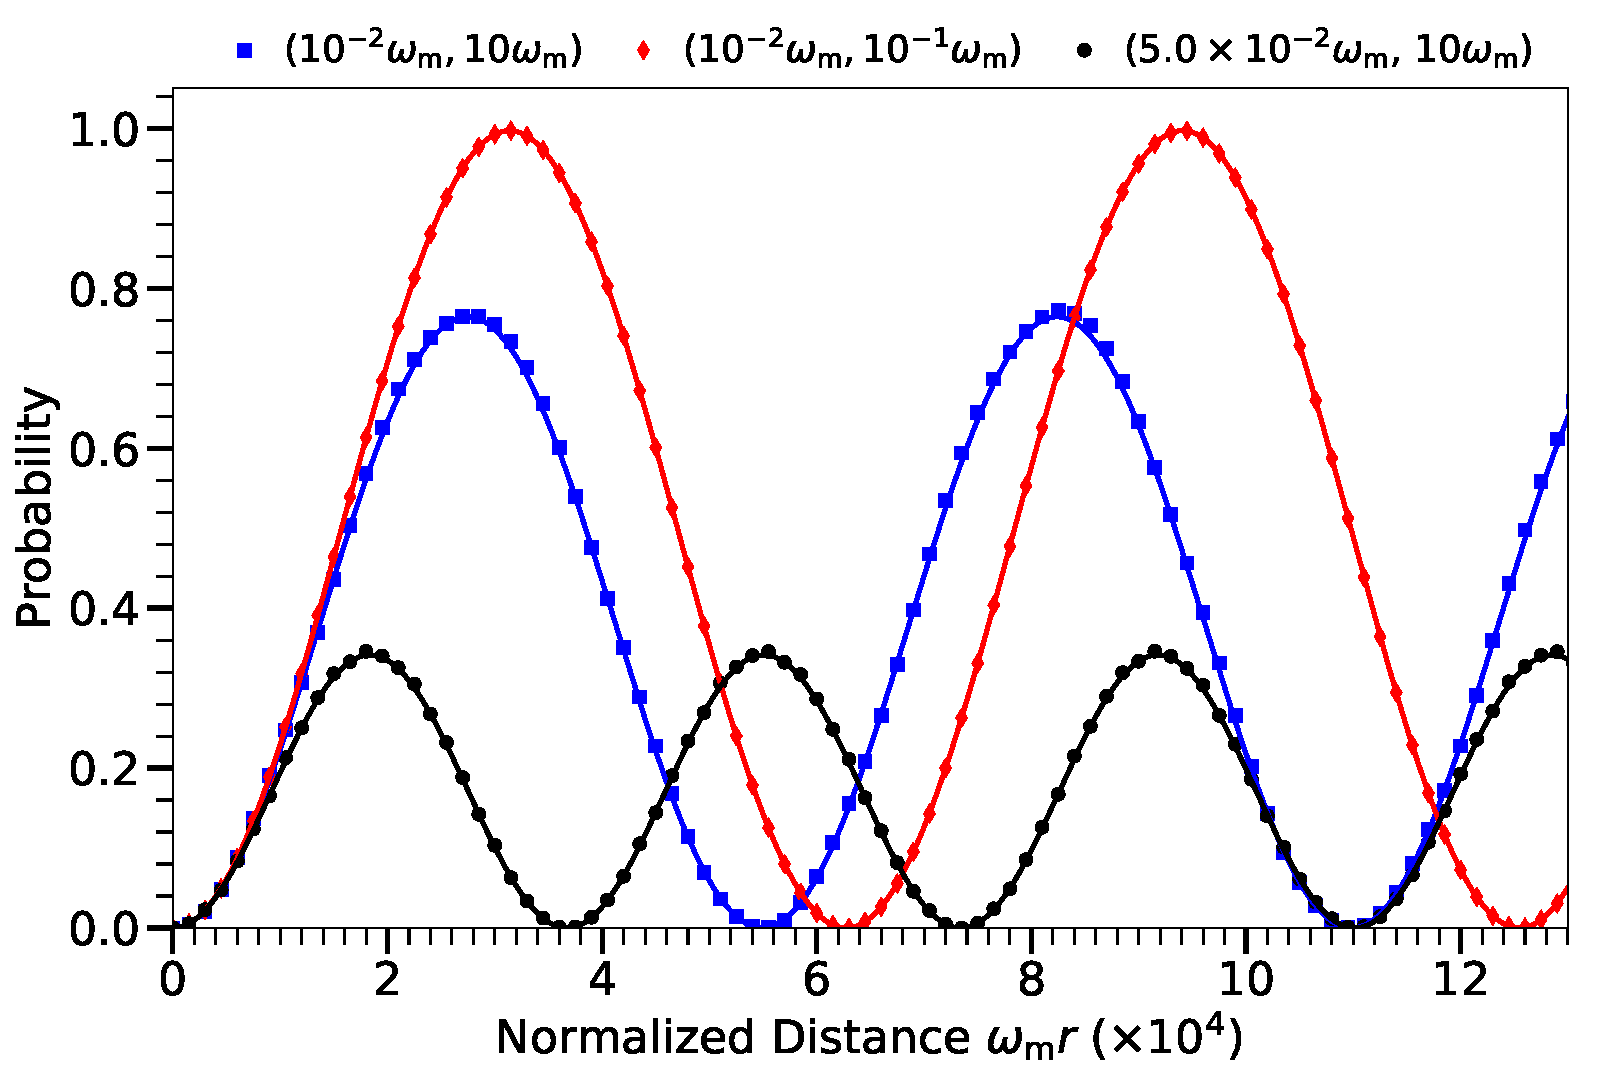
\includegraphics[width=\columnwidth]{chapters/assets/matter/interference-reduction-slide-with-legend}
    \caption{The transition probabilities as functions of distance $r$ for a neutrino propagating through matter profile $\lambda(r) = \lambda_0 + \lambda_1 \cos (k_1 r) + \lambda_2 \cos (k_2 r)$ with different values of $\lambda_2$ and $k_2$ as labeled. The markers are for the numerical results obtained by using the Hamiltonian in Eqn.~\ref{eq-hamiltonian-bg-matter-basis-multi-frequency}, and the continuous curves are obtained using the Rabi formula in Eqn.~\ref{app:rabi-system-transition-probability} but with the values of the modified relative detunings $\RD'_{2+}$ in Table~\ref{table:multi-frequency-rabi-simple-relative-detuning-destruction}. In all three cases, $\lambda_0$ is half of the MSW resonance potential, $\lambda_1/\omega_\mm = 5.2\times 10^{-4}$ and $k_1/\omega_\mm = 1$.}
    \label{fig-rabi-oscillations-energy-gap-change}
\end{figure}

The presence of the additional Fourier mode can suppress the Rabi resonance. This is illustrated in Fig.~\ref{fig-rabi-oscillations-energy-gap-change}. In this figure, I choose the $1+$ Rabi mode to be exactly on resonance with $\lambda_1/\omega_\mm=5.2\times 10^{-4}$ and $k_1/\omega_\mm=1$. The triangles represent the numerical solution for neutrino flavor transformation with $\lambda_2/\omega_\mm=0.052$ and $k_2/\omega_\mm=0.1$. One can see that the transition amplitude is suppressed due to the presence of the second Fourier mode. I used Eqn.~\ref{app:chap:matter-eq:relative-detuning-changed} to calculate the modified relative detunings by taking into account only the $1+$ mode and another Rabi mode. The values of the relative detunings are listed in Table~\ref{table:multi-frequency-rabi-simple-relative-detuning-destruction}. I calculated the transition probability using the Rabi formula in Eqn.~\ref{app:rabi-system-transition-probability} with the relative detuning $\RD'_{2+}$ (the continuous curve in the figure, and it agrees with the numerical solution very well. I also showed two additional examples with $(\lambda_2/\omega_\mm, k_2/\omega_\mm)$ being $(0.052, 10)$ and $(0.26, 10)$, respectively. In both examples, the numerical solutions and the analytic results by using the Rabi formula have excellent agreement.

% To verify the condition, I choose the first Rabi mode to satisfy the resonance condition $k_1=\omega_{\mathrm{m}}$, the condition for the second Rabi mode shifting the system out of resonance is that the relative detuning becomes larger than $1$, which leads to
% \begin{equation}
% \lvert A_2 \rvert \geq \sqrt{2 \lvert A_1 (k_2-\omega_{\mathrm m})\rvert} \equiv A_{2,\mathrm{Critical}}.
% \end{equation}
% I expect the transition amplitude to decrease as we have larger $\lvert A_2\rvert$.

\begin{table}
    \centering
    % \begin{ruledtabular}
    \small
    \setlength\tabcolsep{7pt}
    \begin{tabular}{c | c | c | c | c }
    \hline
    \hline
        $\lambda_2/\omega_\mm$ & $k_2/\omega_\mm$  & $D'_{1-}$ & $D'_{2+}$ & $D'_{2-}$ \\
    \hline
    $0.052$ & $0.1$ & $2.5\times 10^{-5}$ & 0.56 & 0.46 \\
    $0.052$ &  $10$ & $2.5\times 10^{-5}$ & 0.056 & 0.045  \\
    $0.26$ & $10$ &  $2.5\times 10^{-5}$ & 1.4 & 1.1 \\
    \hline
    \hline
    \end{tabular}
    % \end{ruledtabular}
    \caption{\label{table:multi-frequency-rabi-simple-relative-detuning-destruction}The relative detunings of the Rabi resonance when only the $1+$ mode and another Rabi mode are considered.}
\end{table}
% \begin{table}
%     \centering
%     % \begin{ruledtabular}
%     \small
%     \setlength\tabcolsep{2pt}
%     \begin{tabular}{c | c c | cc | cc}
%     \hline
%         \multicolumn{1}{c|}{ $(\lambda_2 \sin(2\theta_\mm)/2, k_2)$ } & \multicolumn{2}{c|}{$(A_{1-}, k_{1-})$} & \multicolumn{2}{c|}{$(A_{2+}, k_{2+})$} & \multicolumn{2}{c}{$(A_{2-}, k_{2-})$} \\
%     \hline
%        & $\RD$ &  Amplitude  & $\RD$ &  Amplitude   & $\RD$ &  Amplitude  \\
%     \hline
%     $(10^{-2}\omega_\mm, 10^{-1}\omega_{\mm})$ &  $2.5\times 10^{-5}$ & 1  &   0.5556 & 0.76   &  0.455 & 0.83 \\
%     $(10^{-2}\omega_\mm, 10\omega_{\mm})$&  $2.5\times 10^{-5}$ & 1  & 0.056 &  1  & 0.045 & 1 \\
%      $(5\times 10^{-2}\omega_\mm, 10\omega_{\mm})$ &  $2.5\times 10^{-5}$ & 1  &  1.389 & 0.34   & 1.136 & 0.44 \\
%     \hline
%     \end{tabular}
%     % \end{ruledtabular}
%     \caption{\label{table:multi-frequency-rabi-simple-relative-detuning-destruction}Relative detuning and oscillation amplitude of each mode for the two-frequency matter profiles.}
% \end{table}



% I choose the two Fourier modes in matter profile so that the first one leads to Rabi mode amplitude $A_1 = \lambda_1 \sin(2\theta_\mm)/2 = 10^{-4}\omega_{\mathrm{m}}$ and frequency $k_1 = \omega_{\mathrm{m}}$. With a small amplitude of the second frequency, $A_2 = \lambda_2 \sin(2\theta)/2  =10^{-4}\omega_{\mathrm{m}}$, and large frequency $k_2=10\omega_{\mathrm{m}}$, I obtain almost full resonance. 
% The relative detuning due to each mode is shown in Table~\ref{table:multi-frequency-rabi-simple-relative-detuning-destruction}
% As shown in Eqn.~\ref{app:chap:matter-eq:relative-detuning-changed}, larger $A_2$ leads to more effective destruction effect. In Fig.~\ref{fig-rabi-oscillations-energy-gap-change}, I am showing the full numerical solution of neutrino oscillations in two-frequency matter background, and the prediction of oscillations using Rabi formula, which is a good match to the numerical results. To show the importance of relative detuning, I also calculated the relative detuning for each cases in Table~\ref{table:multi-frequency-rabi-simple-relative-detuning-destruction}. The Rabi mode with $A_{2+}$ and $k_{2+}$ is always the most destructive one, which is the reason we only use this Rabi mode and the resonance mode to calculate the overall relative detuning and Rabi formula. % Notice that the width of each cases doesn't change since I kept $A_1$ fixed for each calculation, which indicates that the decreasing in transition amplitude is because of the increasing in detuning.



% \subsection{\label{chap:matter-sec:constructive}Constructive Effects}


% Adding a second frequency to the matter density profile can also be constructive.
% I calculated an example with two frequencies in matter density profile, so that the Hamiltonian is
% \begin{equation*}
%     \mathsf H^{(\mm)} = - \frac{\omega_{\mathrm m}}{2} \sigma_3 - \left(\frac{A_1}{2}\cos(k_1 r) + \frac{A_2}{2}\cos(k_2 r) \right) \sigma_1 + \left( \frac{A_1}{2}\sin(k_1 r) + \frac{A_2}{2}\sin(k_2 r) \right) \sigma_2.
% \end{equation*}
% I choose two matter profile frequencies that are off resonance and are producing large relative detunings,
% k1_0.95_k2_2.6_a1_0.025_a2_0.4
% \begin{equation}
%     A_1 = 10^{-4}, \qquad k_1 = 1-10^{-4}, \qquad A_2 = 0.02, \qquad k_2 = 3.
% \end{equation}
% The oscillation amplitude for each mode being much smaller than 1. However, the system produces oscillations are resonance (c.f.~Fig.~\ref{chap:matter-sec:constructive-fig:two-frequencies-constructive}). Using the criteria in Eqn.~\ref{chap:matter-sec:single-frequency-eqn:criterion-for-a2}, I can determine that the Rabi mode with amplitude $A_{2+}=0.02$ and $k_{2+}=3$ is the most important one, which is combined with the one that is closest to resonance $A_{1+}$ to produce relative detuning $\RD = 0$. This argument is consistent with the results shown in Fig.~\ref{chap:matter-sec:constructive-fig:two-frequencies-constructive}.

\begin{figure}[!htbp]
    \centering
    % 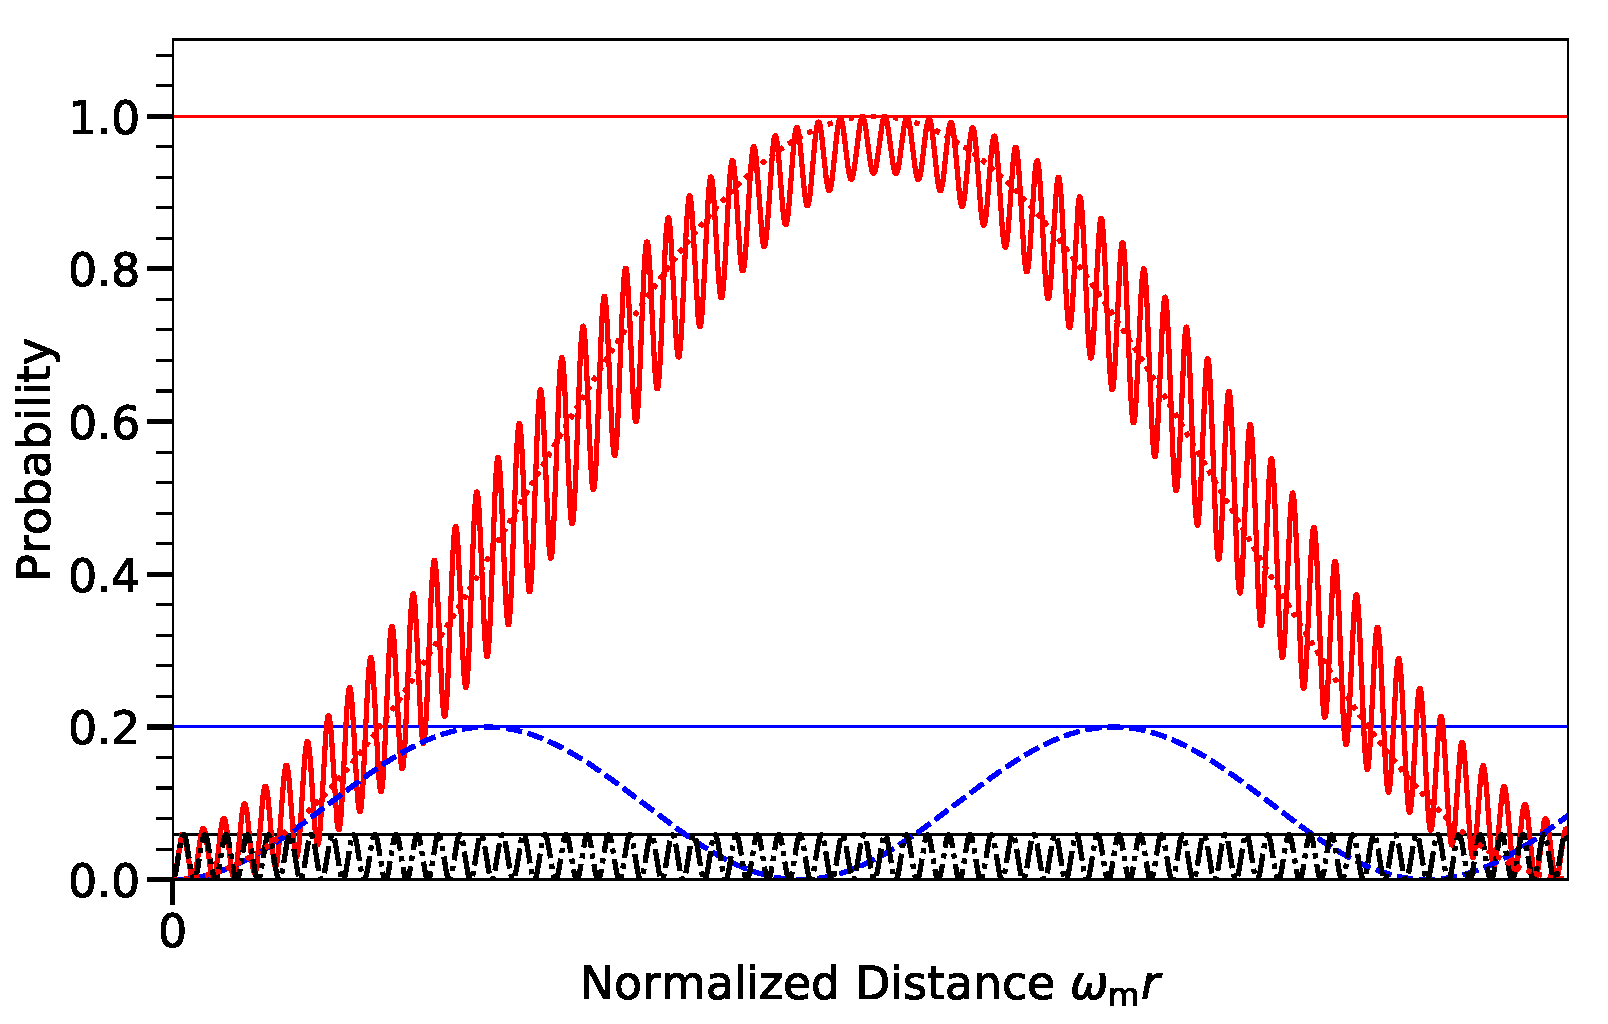
\includegraphics[width=\textwidth]{chapters/assets/rabi/rabiOscillationsNeutrinoCoincidence-two-frequencies-constructive.pdf}
    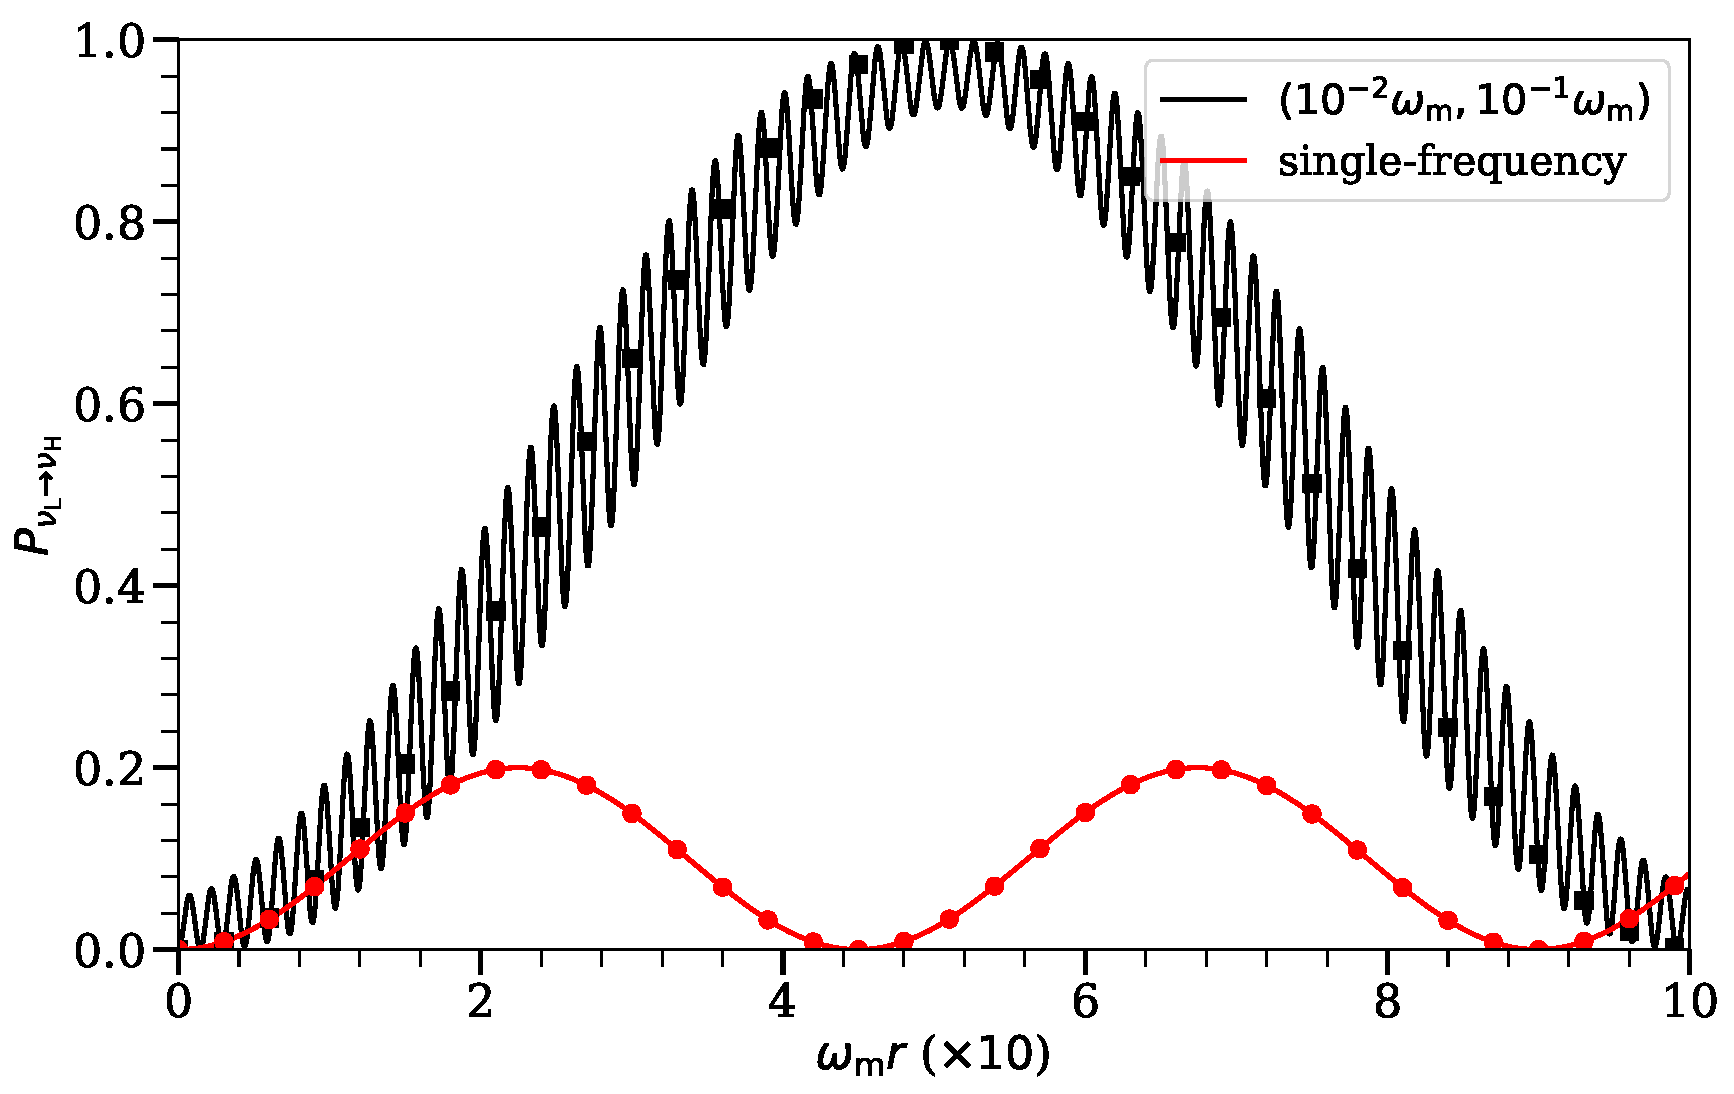
\includegraphics[width=\textwidth]{chapters/assets/matter/interference-enhance-slide-with-legend}
    \caption{The constructive interference effect for the neutrino flavor conversion with a two-frequency matter density profile as in Fig.~\ref{fig-rabi-oscillations-energy-gap-change}. The red dots represent the numerical solution in the case of a single-frequency matter profile with $\lambda_1 /\omega_\mm = 5.2\times 10^{-4}$ and $k_1/\omega_\mm = 1- 10^{-4}$. The black square markers represent the numerical solution with an additional Fourier mode with $\lambda_2/\omega_\mm=0.1$ and $k_2/\omega_\mm=3$. The black curve is obtained using the Rabi formula in Eqn.~\ref{app:rabi-system-transition-probability} with relative detuning $\RD'_{2+}=0$.}
    \label{chap:matter-sec:constructive-fig:two-frequencies-constructive}
\end{figure}

The presence of the second Fourier mode can also enhance the Rabi resonance, which is illustrated in Fig.~\ref{chap:matter-sec:constructive-fig:two-frequencies-constructive}. The two Fourier modes in this figure have amplitudes and wave numbers
\begin{align*}
    \lambda_1/\omega_\mm & =5.2\times 10^{-4}, & k_1/\omega_\mm &= 1- 10^{-4},\\
    \lambda_2/\omega_\mm & =0.1, & k_2/\omega_\mm &= 3,
\end{align*}
respectively. The neutrino flavor conversion is never complete if only the first Fourier mode is present because the relative detuning $\RD_{1+}=1 > 0$. This is shown as the red dots in the figure. However, complete neutrino flavor conversion when both Fourier modes are present. This is because the modified relative detuning $\RD'_{2+} = 0$ when only the $1+$ and the $2+$ Rabi modes are considered. The numerical solution and the analytic prediction using the Rabi formula are plotted as the black squares and the continuous curve, respectively, which agree very well.


%%%%%%%%%%%%%%%%%%%%%%%%%%%%%%%%%%%%%%%%%%%%%%%%%%%%
%%%%%%%%%  Jacobi Anger Expansion  %%%%%%%%%%%%%%%%%%%
%%%%%%%%%%%%%%%%%%%%%%%%%%%%%%%%%%%%%%%%%%%%%%%%%%%%

% \section{\label{sec:jacobi}Rabi Basis and Jacobi-Anger expansion}


% With the intuition of the Rabi oscillations itself as well as the interference between different modes of Rabi oscillations shown in Sec.~\ref{chap:matter-sec:multiple-matter-frequencies}, I can interpret the transition probabilities of any matter profile more precisely if the system can be exactly decomposed into multiple Rabi oscillations. Kneller et al. provided a method to achieve this goal~\cite{Kneller2013}, namely the Jacobi-Anger expansion. While they used the Jacobi-Anger expansion to calculate the neutrino oscillations in single frequency matter profiles through complicated calculation, I use a different approach that motivates us to use the Jacobi-Anger expansion and simplifies the concepts and calculations. In this section, I will first show that a better basis can be found for the interpretation of neutrino oscillations in matter. Then, I will show that the neutrino oscillations in matter can be decomposed into superpositions of Rabi oscillations by applying the Jacobi-Anger expansion.


\section{\label{chap:matter-sec:jacobi-subsec:rabi-basis}Rabi Basis}

Previously I have ignored the oscillating $\sigma_3$ terms in the Hamiltonian such as in Eqn.~\ref{chap:matter-sec:single-fequency-eq:hamiltonian-bg-matter-basis-single-frequency}. Using the Jacobi-Anger expansion, J. Kneller et al. showed that these terms result in an infinite number of resonance conditions. In the rest of the chapter, I will present a much simpler derivation of their results from the perspective of Rabi oscillations. For this purpose I will define a new basis called Rabi basis
\begin{equation}
\begin{pmatrix} \ket{\nu_{\mathrm{r1}}}\\ \ket{\nu_{\mathrm{r2}}} \end{pmatrix} =  \mathsf{U}^\dagger \begin{pmatrix} \ket{\nu_{\mathrm{L}}} \\ \ket{\nu_{\mathrm{H}}} \end{pmatrix},
\label{eq-rabi-basis}
\end{equation}
where 
\begin{equation}
\mathsf{U} =  \begin{pmatrix} e^{-\ri \eta (r)} & 0 \\  0 & e^{\mathrm i \eta (r)}  \end{pmatrix}.
\label{eq-rabi-transformation}
\end{equation}
The unitary transformation in Eqn.~\ref{eq-rabi-transformation} is a rotation in flavor space about the third axis.
% with generator $\exp\left(-\mathrm i\frac{\sigma_3}{2}\cdot 2\eta\right)$,
It commutes with $\sigma_3$ terms in the Hamiltonian, but, due to its dependence on $r$, the left side of the Schr\"{o}dinger equation obtains an extra term:
%other than the derivative, which can be used to cancel the varying $\sigma_3$ term, i.e., $\delta\lambda(r) \cos 2\theta_{\mathrm m} \sigma_3/2$. In the flavor isospin picture, the transform brings the neutrino states into a rotating frame so that the varying energy gap due to the fluctuating matter density is exactly cancelled by rotation of the frame.
% By remove the varying $\sigma_3$ term in this way, the energy gap in the Rabi basis becomes a constant energy gap.
% Another advantage of this transformation is that the transition probability from light state to heavy state in background matter basis is easily calculated as $P_{\mathrm{L} \to \mathrm{H}} (x) = \lvert e^{i\eta} \psi_{\mathrm r2} (x)  \rvert^2 = \lvert \psi_{\mathrm r2} (x)  \rvert^2$. One can easily show that the transition probability between two eigenstates in the Rabi basis is the same as the transition probability between two eigenstates in background matter basis, given the initial condition that the system is in low energy state.
% In the Rabi basis, the Schr\"{o}dinger equation is
\begin{align*}
    &\begin{pmatrix}  \frac{\mathrm d\eta}{\mathrm dr}  & 0 \\ 0 & - \frac{\mathrm d\eta}{\mathrm d r}  \end{pmatrix} \begin{pmatrix} \psi_{\mathrm R1} \\ \psi_{\mathrm R2} \end{pmatrix} + \mathrm i \frac{\mathrm d}{\mathrm dr} \begin{pmatrix} \psi_{\mathrm R1} \\ \psi_{\mathrm R2} \end{pmatrix} \\
    =& \left[ -\frac{\omega_{\mathrm m} }{2} \sigma_3  + \frac{\delta \lambda}{2} \cos 2\theta_{\mathrm m}  \sigma_3  - \frac{\delta \lambda}{2} \sin 2\theta_{\mathrm m} \begin{pmatrix} 0 & e^{2\mathrm i\eta} \\ e^{-2 \mathrm i\eta } & 0 \end{pmatrix}   \right] \begin{pmatrix} \psi_{\mathrm R1} \\ \psi_{\mathrm R2} \end{pmatrix}.
\end{align*}
The oscillating $\sigma_3$ terms in Hamiltonian can be eliminated by choosing $\eta(r)$ properly, i.e.,
\begin{equation}
    \eta(r) - \eta(0) =  \frac{\cos 2\theta_{\mathrm{m}}}{2} \int_0^r \delta\lambda (\tau) \dd\tau.
\end{equation}
With this definition, the Schr\"{o}dinger equation simplifies:
\begin{equation}
    \ri \frac{\dd}{\dd r} \begin{pmatrix} \psi_{\mathrm r1} \\ \psi_{\mathrm r2} \end{pmatrix} = \left[ - \frac{\omega_{\mathrm m}}{2} \sigma_3 - \frac{\delta \lambda}{2} \sin 2\theta_{\mathrm m} \begin{pmatrix} 0 & e^{2\ri\eta} \\ e^{-2 \ri \eta } & 0 \end{pmatrix}\right] \begin{pmatrix} \psi_{\mathrm r1} \\ \psi_{\mathrm r2} \end{pmatrix}.
    \label{chap:matter-sec:jacobi-subsec:rabi-basis-eqn:eom-rabi-basis-matter}
\end{equation}
Because the states $\ket{\nu_{r1}}$ and $\ket{\nu_{r2}}$ are related to $\ket{\nu_{\mathrm L}}$ and $\ket{ \nu_{\mathrm H} }$ by phase factors only, the transition probability between the former two states is the same as that between the latter.



\section{\label{chap:matter-sec:single-revisted}Single-Frequency Matter Profile Revisited}
% \subsection{\label{chap:matter-sec:jacobi-subsec:jacobi}Jacobi-Anger Expansion}


% For a rigorous analysis of neutrino oscillations in oscillatory matter profiles, I will need the Jacobi-Anger expansion. Jacobi-Anger expansion is used to expand exponential functions of the form $e^{\ri r \sin (\phi)}$ using the basis $e^{\ri n \phi }$,
% \begin{equation}
% e^{\ri r \sin (\phi)} = \sum_{n=-\infty}^\infty  J_n(r) e^{\ri n\phi}.
% \end{equation}
% J. Kneller and K. Patton et al. used this method to calculate the transition probabilities of neutrinos in oscillatory matter profile~\cite{Kneller2010,Kneller2013,Patton2014}. In this subsection, I will review the method of Jacobi-Anger expansion and its application to neutrino oscillations, using a different formalism. 

Let us consider the single-frequency matter profile that we have studied in Sec.~\ref{chap:matter-sec:single} again. In the Rabi basis, the Hamiltonian becomes
\begin{equation}
    \mathsf H^{(\RR)} = \frac{\omega_\mm}{2} \sigma_3 - \frac{\sin 2\theta_\mm \lambda_1\cos (k_1 r)}{2} \begin{pmatrix}
        0 & e^{2\ri \eta(r)} \\
        e^{-2\ri \eta(r)} & 0
    \end{pmatrix},
\end{equation}
where
\begin{equation}
    \eta(r) =  \frac{\lambda_1 \cos 2\theta_{\mathrm m}}{2 k} \sin (k_1 r) .
\end{equation}
With the Jacobi-Anger expansion
\begin{equation}
e^{\ri z \sin (\phi)} = \sum_{n=-\infty}^\infty  J_n(z) e^{\ri n\phi},
\end{equation}
the term $e^{2\ri \eta(r)}$ becomes
\begin{equation}
    \exp\left({\ri \frac{\lambda_1 \cos 2\theta_{\mm}}{k_1} \sin (k_1 r) }\right)  =  \sum_{n=-\infty}^{\infty} J_n \left( \frac{\lambda_1 \cos 2\theta_\mm}{k_1}\right) e^{\ri n k_1 r},
\end{equation}
and  the Hamiltonian becomes a Rabi oscillation system with infinite number of Rabi modes:
\begin{equation}
    \mathsf H^{(\mathrm{R})} =
    -\frac{\omega_{\mathrm{m}}}{2} \sigma_3
    -  \frac{1}{2} \sum_{n=-\infty}^\infty A_n \begin{pmatrix}
    0 &  e^{\ri n k_1  r} \\
     e^{ - \ri n k_1 r} & 0
    \end{pmatrix},
    \label{chap:matter-sec:jacobi-eqn:hamil-jacobi-expanded}
\end{equation}
where $J_n(z)$ is the Bessel function of the first kind of order $n$, and
\begin{align}
    A_n &= \tan 2\theta_{\mathrm m} n k_1 J_{n} \left( \frac{\lambda_1}{k_1}\cos 2\theta_{\mathrm m} \right)
\end{align}
and $n k_1$ are the amplitude and wave number of the $n$th Rabi mode.\footnote{A phase in the matter potential would contribute to the phases of the Rabi modes which do not play any role in the resonance for the reason discussed in Sec.~\ref{chap:app-sec:rabi-oscillations}}
In obtaining Eqn.~\ref{chap:matter-sec:jacobi-eqn:hamil-jacobi-expanded}, I have used the following identify of the Bessel function
\begin{equation}
    J_{n-1}(z) + J_{n+1}(z) = \frac{2 n}{z} J_n(z).
    \label{eqn:bessel-function-sum-property}
\end{equation}


Eqn.~\ref{chap:matter-sec:jacobi-eqn:hamil-jacobi-expanded} implies an infinite number of resonance conditions
\begin{equation}
    \omega_\mm  = n k_1 \qquad (n=1, 2, \ldots)
    \label{chap:matter-sec:single-revisted-eqn:resonance-condition}
\end{equation}
However, the amplitude of the Rabi mode $A_n$ drops quickly as a function of $n$ because
\begin{equation}
    J_n(z) \xrightarrow{z\ll \sqrt{n+1}} \frac{ (z/2)^n }{n!} \qquad \text{if } n>0
    % J_1\left( \frac{\lambda_1}{k_1}\cos (2\theta_{\mathrm m}) \right) \approx \frac{\lambda_1}{2k_1}\cos (2\theta_{\mathrm m})
    \label{chap:matter-sec:single-revisit-eqn:bessel-small-arg}
\end{equation}
when $\lambda_1/k_1 \ll 1$. For $\lambda_1/k_1\gtrsim 1$, $A_n$ also becomes small for sufficiently large $n$ because
\begin{equation}
    J_n(z) \xrightarrow{n\gg 1} \frac{1}{\sqrt{2\pi n}} \left( \frac{ e z }{ 2n } \right)^n.
% J_n(n \sech \alpha) \sim \frac{ e^{n(\tanh\alpha - \alpha)} }{\sqrt{ 2\pi n \tanh \alpha } }
\end{equation}
Any real physical system has a finite size $l$ and the Rabi modes with the oscillation wavelengths $2\pi/\Omega_n\sim 2\pi/A_n  \gtrsim l$ can be ignored even if they are on resonance.




% When the matter interaction provides one dominate resonance mode and without significant interference between the resonance mode and the other modes, all off-resonance modes can be dropped as an approximation. To be precise, as I have shown previously in Sec.~\ref{chap:app-sec:rabi-oscillations}, interference might happen between different modes and there exists a criterion for it to be important. 
% First of all, I will explain the approximations used in Eqn.~\ref{eq-hamiltonian-bg-matter-basis-single-frequency} to simplify the Hamiltonian.
% Even for the single frequency matter profile, there are two Rabi modes $\pm k_1$, under the approximation that the varying $\sigma_3$ term in Hamiltonian is neglected, as mentioned in Sec.~\ref{chap:app-sec:rabi-oscillations}. The three examples calculated in Fig.~\ref{fig-rabiOscillationsNeutrinoCoincidence} are almost exact since the modification of relative detuning for the $k_1$ mode that we kept, due to the far off resonance mode $-k_1$ that I neglected, is tiny. Since I have derived the interference effect in Sec.~\ref{chap:app-sec:rabi-oscillations}, the approximations can be justified quantitatively using Eqn.~\ref{app:chap:matter-eq:relative-detuning-changed}.

% In order for a Rabi mode to have significant effect on the transition probabilities, it requires a small relative detuning $\RD$, and a reasonable oscillation wavelength compared to the size of the physical system. The relative detuning for each mode is calculated as
% \begin{equation}
% \RD_n = \frac{\lvert n k_1 - \omega_{\mathrm{m}} \rvert}{A_n}
% \end{equation}
% for single frequency matter profile.
% % , and
% % \begin{equation}
% % \RD_{\{n_a\}} = \frac{\lvert \sum_a n_a k_a -\omega_{\mathrm m} \rvert }{A_{\{n_a\}}}
% % \end{equation}
% % for multi-frequency matter profile.
% For the Rabi modes with small relative detunings, they are important since they might lead to full transition. However, the full transition requires at least some distance comparable to the wavelength of the oscillation. Suppose I have a Rabi mode that has zero relative detuning, but with a oscillation wavelength that is much larger than the size of the neutrino oscillations system, such a Rabi mode would never have the time to accumulate a large transition probability within the region of interest. 
% %The Rabi oscillation shows that the oscillation wavelength of each mode is determined by the Rabi frequency
% % \begin{equation}
% % \Omega_{\{n_a\}} = \lvert A_{\{n_a\}} \rvert \sqrt{1+\RD_{\{n_a\}}^2}.
% % \end{equation}
% The Rabi modes that has much larger oscillation wavelength are not subjected consideration even though their relative detunings are close to zero. While I can always approximate the oscillations by including as many Rabi modes as possible to approximate the neutrino oscillations, such effort is not always necessary.


% In Table~\ref{tab-q-values-single-frequency-example} I calculated the relative detunings of the three cases in Fig.~\ref{fig-rabiOscillationsNeutrinoCoincidence}, where $n=\pm 1$ are for the $\pm k_1$ modes in the Hamiltonian Eqn.~\ref{eq-hamiltonian-bg-matter-basis-single-frequency}. The $\RD'_1$ is the shifted relative detuning of the first mode with $n=1$ due to other mode. It clearly shows that the first mode takes the whole system so that the approximation of neglecting the varying $\sigma_3$ terms in Hamiltonian is accurate enough. One can also show that the interference effect due to higher order modes is negligible, since they do not change the relative detuning of the most significant modes. It confirms the results I observed in Fig.~\ref{fig-rabiOscillationsNeutrinoCoincidence} that the change of the relative detuning due to the $-k_1$ mode is not observable.

In Sec.~\ref{chap:matter-sec:single}, I have discussed the scenario where the $n=1$ Rabi mode is on or close to resonance and $\lambda_1/\omega_\mm \ll 1$. Using Eqn.~\ref{chap:matter-sec:single-revisit-eqn:bessel-small-arg} and identity
\begin{equation}
    J_{-n}(z) =(-1)^n J_{n}(z)
\end{equation}
I obtain
\begin{equation}
    A_{\pm 1} \approx \frac{ \lambda_1 \sin (2\theta_\mm)}{2},
\end{equation}
which agrees with Eqn.~\ref{chap:matter-sec:single-eqn:rabi-amplitudes}. According to Eqn.~\ref{app:chap:matter-eq:relative-detuning-changed}, compared with the case where the first Rabi mode is present, the relative detuning of the Rabi resonance has a change of magnitude
\begin{equation}
\Delta \RD_{(n)} = \frac{1}{2} \frac{A_n}{A_1} \frac{1}{\RD_n}
\end{equation}
when another Rabi mode $n$ is present, where $\RD_n$ is the relative detuning when only the $n$th Rabi mode is considered. In Table~\ref{table:relative-detunings-single-frequency-example}, I listed the values of $A_n/A_1$, $\RD_n$, and $\Delta \RD_{(n)}$ of a few off-resonance Rabi modes for the three numerical examples plotted in Fig.~\ref{fig-rabiOscillationsNeutrinoCoincidence}. One can see that all the off-resonance Rabi modes have very little impact on the resonance which explains why we could ignore the oscillating $\sigma_3$ terms in Eqn.~\ref{eq-hamiltonian-bg-matter-basis-single-frequency}.



% single frequency matter potential $\lambda = \lambda_0 + \lambda_1 \cos(k_1 r)$ by removing the varying $\sigma_3$ term by arguing that this term has no effect on transition probabilities when the system is close to resonance, $k_1 \sim \omega_{\mathrm m}$. The reason is that only the first mode $n=1$ is on resonance when $k_1=\omega_{\mathrm m}$ and all other modes are far from resonance, thus
% \begin{align}
% \mathsf H^{\mathrm R} \approx & -\frac{\omega_{\mathrm m}}{2}\sigma_3 - \frac{1}{2} A_1 \begin{pmatrix}
% 0 & e^{i k_1 r} \\
% e^{-ik_1r} & 0
% \end{pmatrix}\label{eq-single-frequency-first-mode-hamiltonian} \\
% \approx & -\frac{\omega_{\mathrm m}}{2} \sigma_3 - \frac{A_1}{2} \cos(k_1 r) \sigma_1 + \frac{A_1}{2} \cos(k_1 r) \sigma_2\nonumber,
% \end{align}
% where $A_1$ is defined in Eqn.~(\ref{eq-define-a1}) and approximation
% \begin{equation*}
% J_1\left( \frac{\lambda_1}{k_1}\cos (2\theta_{\mathrm m}) \right) \approx \frac{\lambda_1}{2k_1}\cos (2\theta_{\mathrm m})
% \end{equation*}
% for $\lambda_1\cos(2\theta_{\mathrm m})/k_1\ll 1$ is used in the last step. Thus I obtained the same equation as the one used in Sec.~\ref{chap:matter-sec:single}. $\lambda_1\cos(2\theta_{\mathrm m})/k_1\ll 1$ corresponds to small resonance width for Eqn.~(\ref{eq-hamiltonian-bg-matter-basis-single-frequency}) and also Eqn.~(\ref{eq-single-frequency-first-mode-hamiltonian}) so that the interferences are small by Eqn.~\ref{app:chap:matter-eq:relative-detuning-changed}.


% Using Jacobi-Anger expansion, we can calculate the relative detuning for each mode as well as the interference effect. The relative detuning for each mode in the Jacobi-Anger expansion for single frequency matter profile used in Fig.~\ref{fig-rabiOscillationsNeutrinoCoincidence} is calculated and listed in Table~\ref{tab-q-values-single-frequency-example}. 



% {
%  {{1}, 0.},
%  {{-1}, 103239.},
%  {{2}, 1.11987*10^9},
%  {{-2}, 3.3596*10^9},
%  {{3}, 9.71798*10^13},
%  {{-3}, 1.9436*10^14},
%  {{4}, 9.48722*10^18}
% }
% {324336., 3.14159, 6.28319, 2.0944}

% {
%  {{1}, 1.03239},
%  {{-1}, 103238.},
%  {{2}, 1.1198*10^9},
%  {{-2}, 3.35948*10^9}
% }
% {225656., 3.14162, 6.28356, 2.09446}

% {
%  {{1}, 5.16197},
%  {{-1}, 103234.},
%  {{2}, 1.11953*10^9},
%  {{-2}, 3.35904*10^9}
% }
% {61685., 3.14175, 6.28507, 2.09474}

\begin{table*}
\centering
% \begin{ruledtabular}
\scriptsize
\setlength\tabcolsep{2pt}
\begin{tabular}{r|ccc|ccc|ccc}
\hline
\hline
\multicolumn{1}{r|}{} & \multicolumn{3}{c|}{$k_1/\omega_{\mathrm m}=1$} & \multicolumn{3}{c|}{$k_1/\omega_\mm=1-2\times 10^{-5}$} & \multicolumn{3}{c}{$k_1/\omega_\mm=1-10^{-4}$} \\
\hline
   $n$ & $A_n/A_1$ & $\RD_n$  & $\Delta \RD_{(n)}$  & $A_n/A_1$ & $\RD_n$  & $\Delta \RD_{(n)}$  & $A_n/A_1$ & $\RD_n$  & $\Delta \RD_{(n)}$   \\
\hline
 -1 &	$1$  & $10^5$ &   $5\times 10^{-6}$   & 1 &	$10^{5}$ &  $5\times 10^{-6}$    &	$1$ &  $10^{5}$ & $5\times 10^{-6}$   \\
 2 & $4.8 \times 10^{-5}$ & $1.1 \times 10^{9}$ & $2.2\times 10^{-14}$  & $4.8 \times 10^{-5}$ & $1.1\times 10^9$ & $2.2\times 10^{-14}$ &  $4.8 \times 10^{-5}$ & $1.1\times 10^9$ & $2.2\times 10^{-14}$ \\
 $-2$ &  $4.8 \times 10^{-5}$ & $3.2\times 10^{9}$ & $7.5\times 10^{-15}$  &  $4.8 \times 10^{-5}$ & $3.2\times 10^{9}$ & $7.5\times 10^{-15}$ &   $4.8 \times 10^{-5}$ & $3.2\times 10^{9}$ & $7.6\times 10^{-15}$ \\
\hline
\hline
\end{tabular}
% \end{ruledtabular}
\caption{\label{table:relative-detunings-single-frequency-example}The amplitudes and the relative detunings of a few Rabi modes and their impact on the Rabi resonance for the three numerical examples shown in Fig.~\ref{fig-rabiOscillationsNeutrinoCoincidence}.}
\end{table*}
%%%%%%%%%%%%%%%%%%%%%%%%%%%%%%%%%%%
%%%%% Using data from Mathematica notebook: relative-detunings-in-paper.nb


% \begin{table*}
% \centering
% % \begin{ruledtabular}
% \small
% \setlength\tabcolsep{2pt}
% \begin{tabular}{lccc|lccc|lccc}
% \hline
%  \multicolumn{4}{c|}{$k_1=\omega_{\mathrm m}$} & \multicolumn{4}{c|}{$k_1=(1-2\times 10^{-5})\omega_{\mathrm{m}}$} & \multicolumn{4}{c}{$k_1=(1-10^{-4})\omega_{\mathrm m}$} \\
% \hline
%    $n$ & $\RD$ & $\RD'_1$  & $2\pi\omega_{\mathrm m}/\Omega_n$ & $n$ & $\RD$ & $\RD'_1$ & $2\pi\omega_{\mathrm m}/\Omega_n$ & $n$ & $\RD$ & $\RD'_1$ & $2\pi\omega_{\mathrm m}/\Omega_n$  \\
% \hline
%  1 &	0  & - &   $3.2\times10^5$   & 1 &	1 &  -  &   $2.2\times 10^5$       & 1   &	$5.2$ &  - & $6.2\times10^4$   \\
% -1 &	$10^5$ &  $4.8\times 10^{-6}$  &   $3.1$     &     -1 &	$10^5$ &   1  &   $3.1$               &  -1 &	$10^5$  & $5.2$ & $3.1$  \\
% 2 &	$1.1\times 10^9$  &   $2.1\times 10^{-14}$  &   $6.3$    &  2 & 	$1.1\times 10^9$ &  1  &    $6.3$   &  2  &	$1.1\times 10^9$  &  $5.2$  & $6.3$  \\
% -2 &	$3.4\times 10^9$  & $6.9\times 10^{-15}$ & $2.1$ &    -2 &	$3.4\times10^9$ &  1  &  $2.1$          & -2  &	$3.4\times 10^9$ & $5.2$ &  $2.1$  \\
% \hline
% \end{tabular}
% % \end{ruledtabular}
% \caption{\label{tab-q-values-single-frequency-example}Relative detuning and oscillation wavelength of each mode for single frequency matter profile.}
% \end{table*}


% The impact of detuning is also verified in Fig.~\ref{chap:matter-sec:single-revisted-fig:prob-amp-jacobi-anger}. The example clearly shows the width of the resonance is dropping dramatically for larger modes in Jacobi-Anger expansion. A careful investigation shows that the resonance width is dropping exponentially as shown in Fig.~\ref{chap:matter-sec:single-revisted-fig:resonance-width-jacobi-anger-exp} and Fig.~\ref{chap:matter-sec:single-revisted-fig:resonance-width-heatmap}.




% \begin{figure}[!htbp]
%     \centering
%     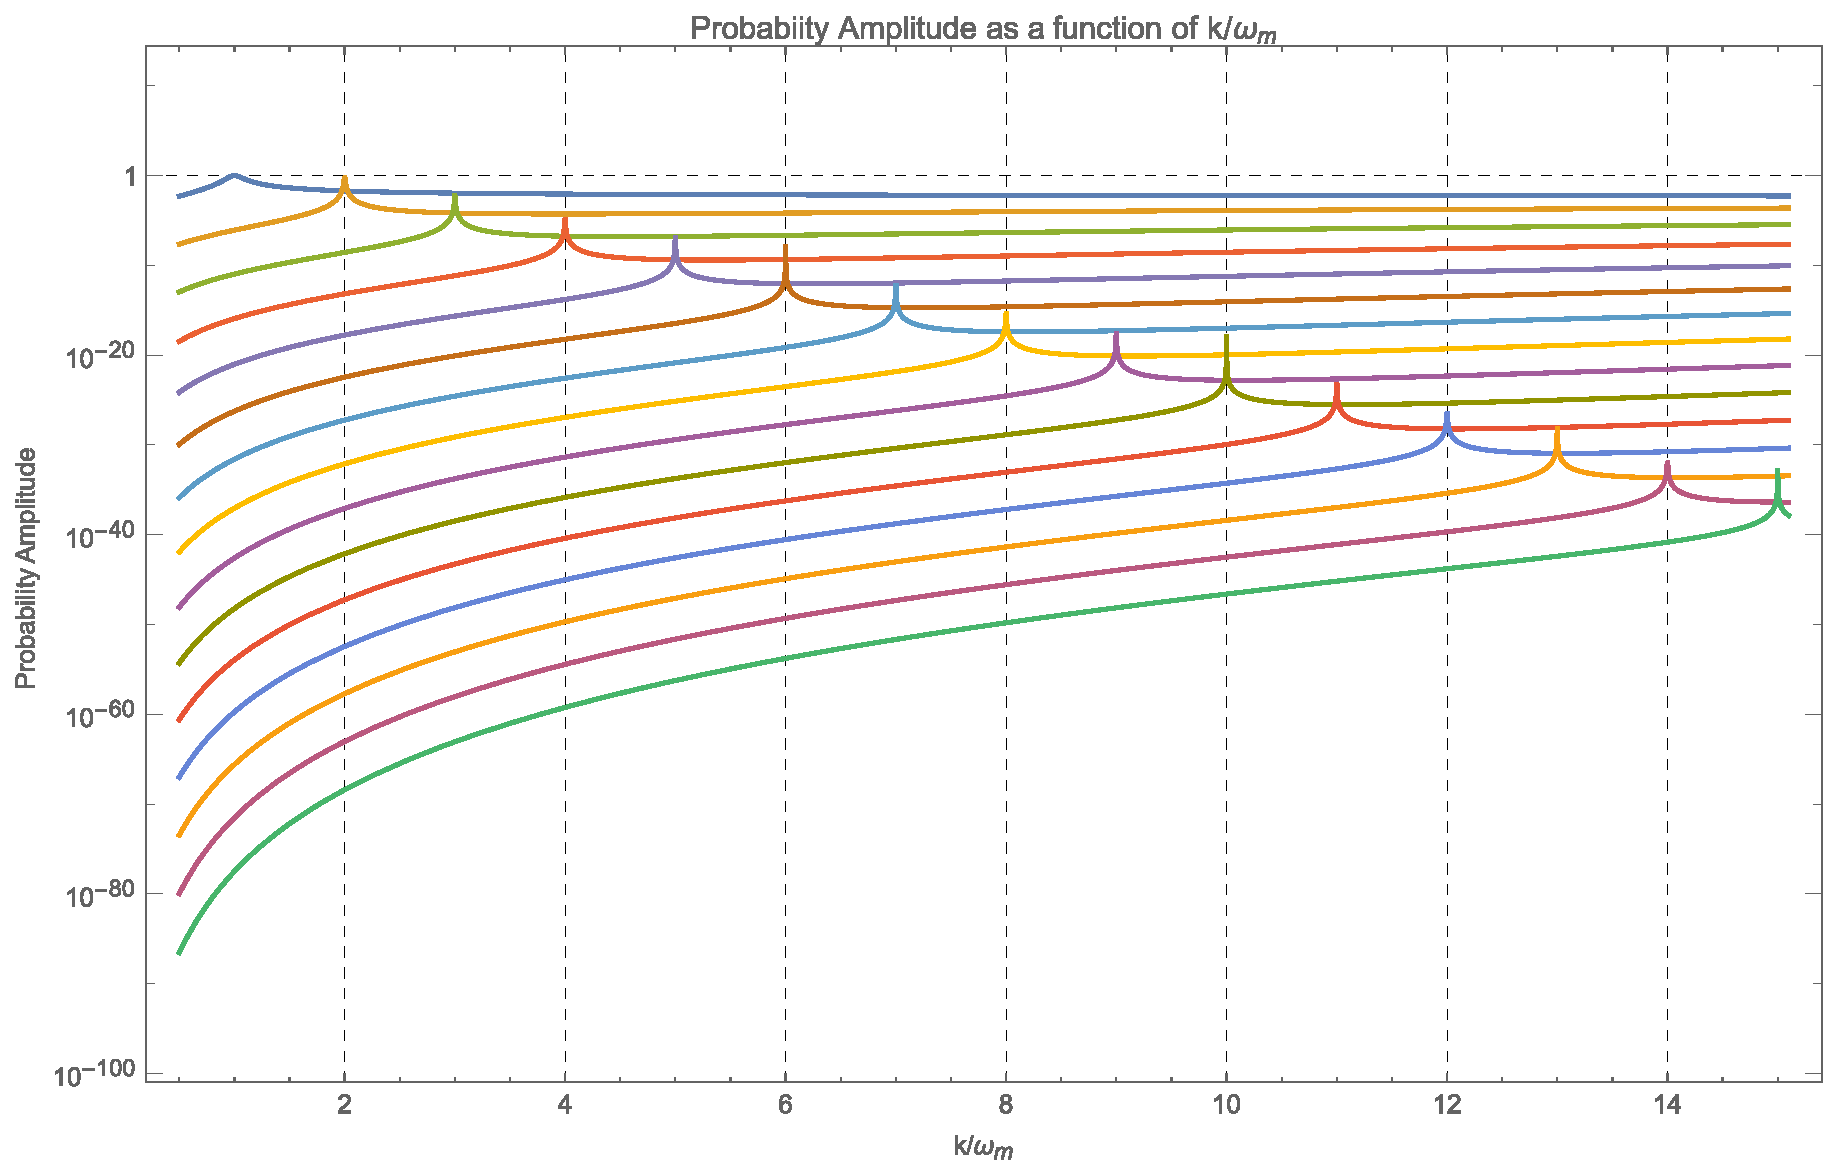
\includegraphics[width=\textwidth]{chapters/assets/rabi/stimulated-probability-apmlitude-vs-k-Jacobi-Anger.pdf}
%     \caption{Probability amplitude as a function of $k/\omega_{\mathrm m}$ for each term in Jacobi-Anger expansion, with parameters $\lambda_1=0.1$,$\theta_{\mathrm m}=\pi/5$.}
%     \label{chap:matter-sec:single-revisted-fig:prob-amp-jacobi-anger}
% \end{figure}


% \begin{figure}[!htbp]
%     \centering
%     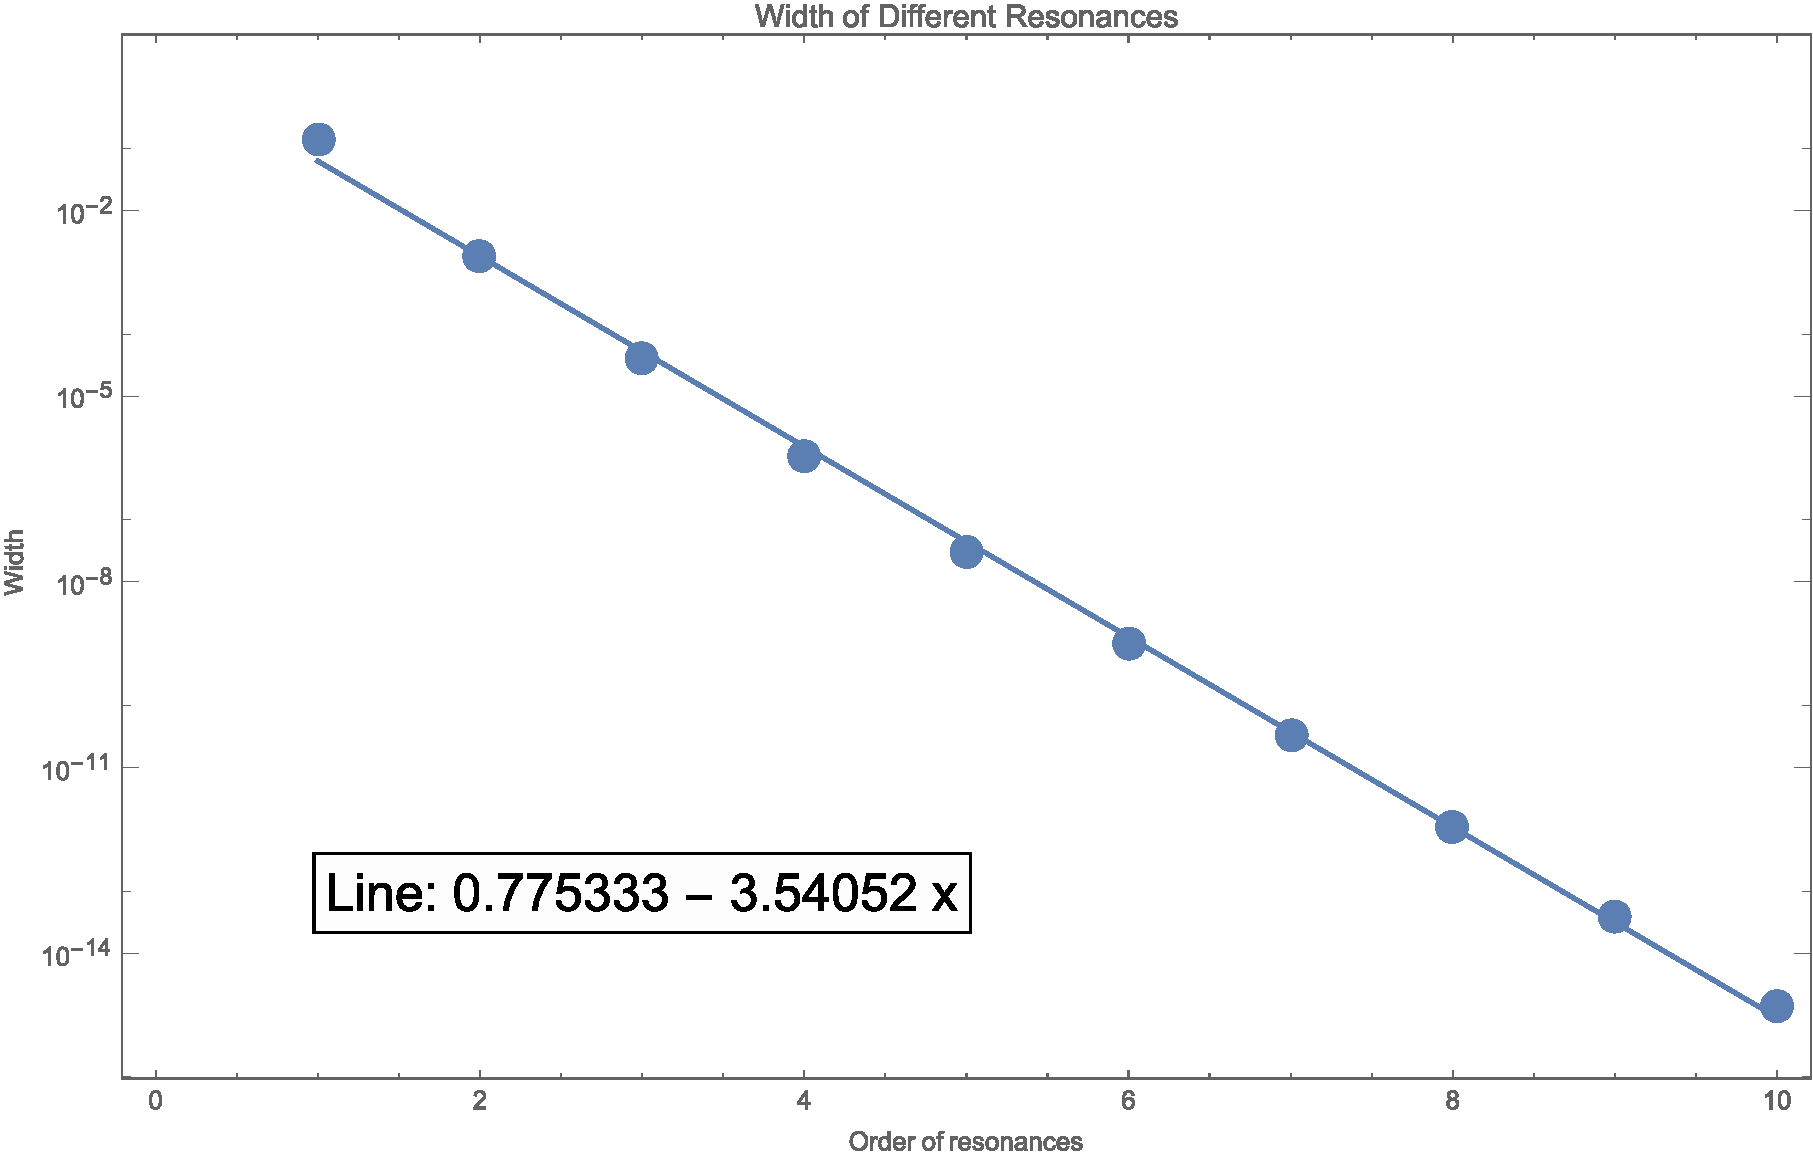
\includegraphics[width=\textwidth]{chapters/assets/rabi/stimulated-probability-apmlitude-vs-k-resonance-width.pdf}
%     \caption{Resonance width as a function of mode order for each term in Jacobi-Anger expansion, with parameters $\lambda_1=0.1$,$\theta_{\mathrm m}=\pi/5$.}
%     \label{chap:matter-sec:single-revisted-fig:resonance-width-jacobi-anger-exp}
% \end{figure}



% \begin{figure}[!htbp]
%     \centering
%     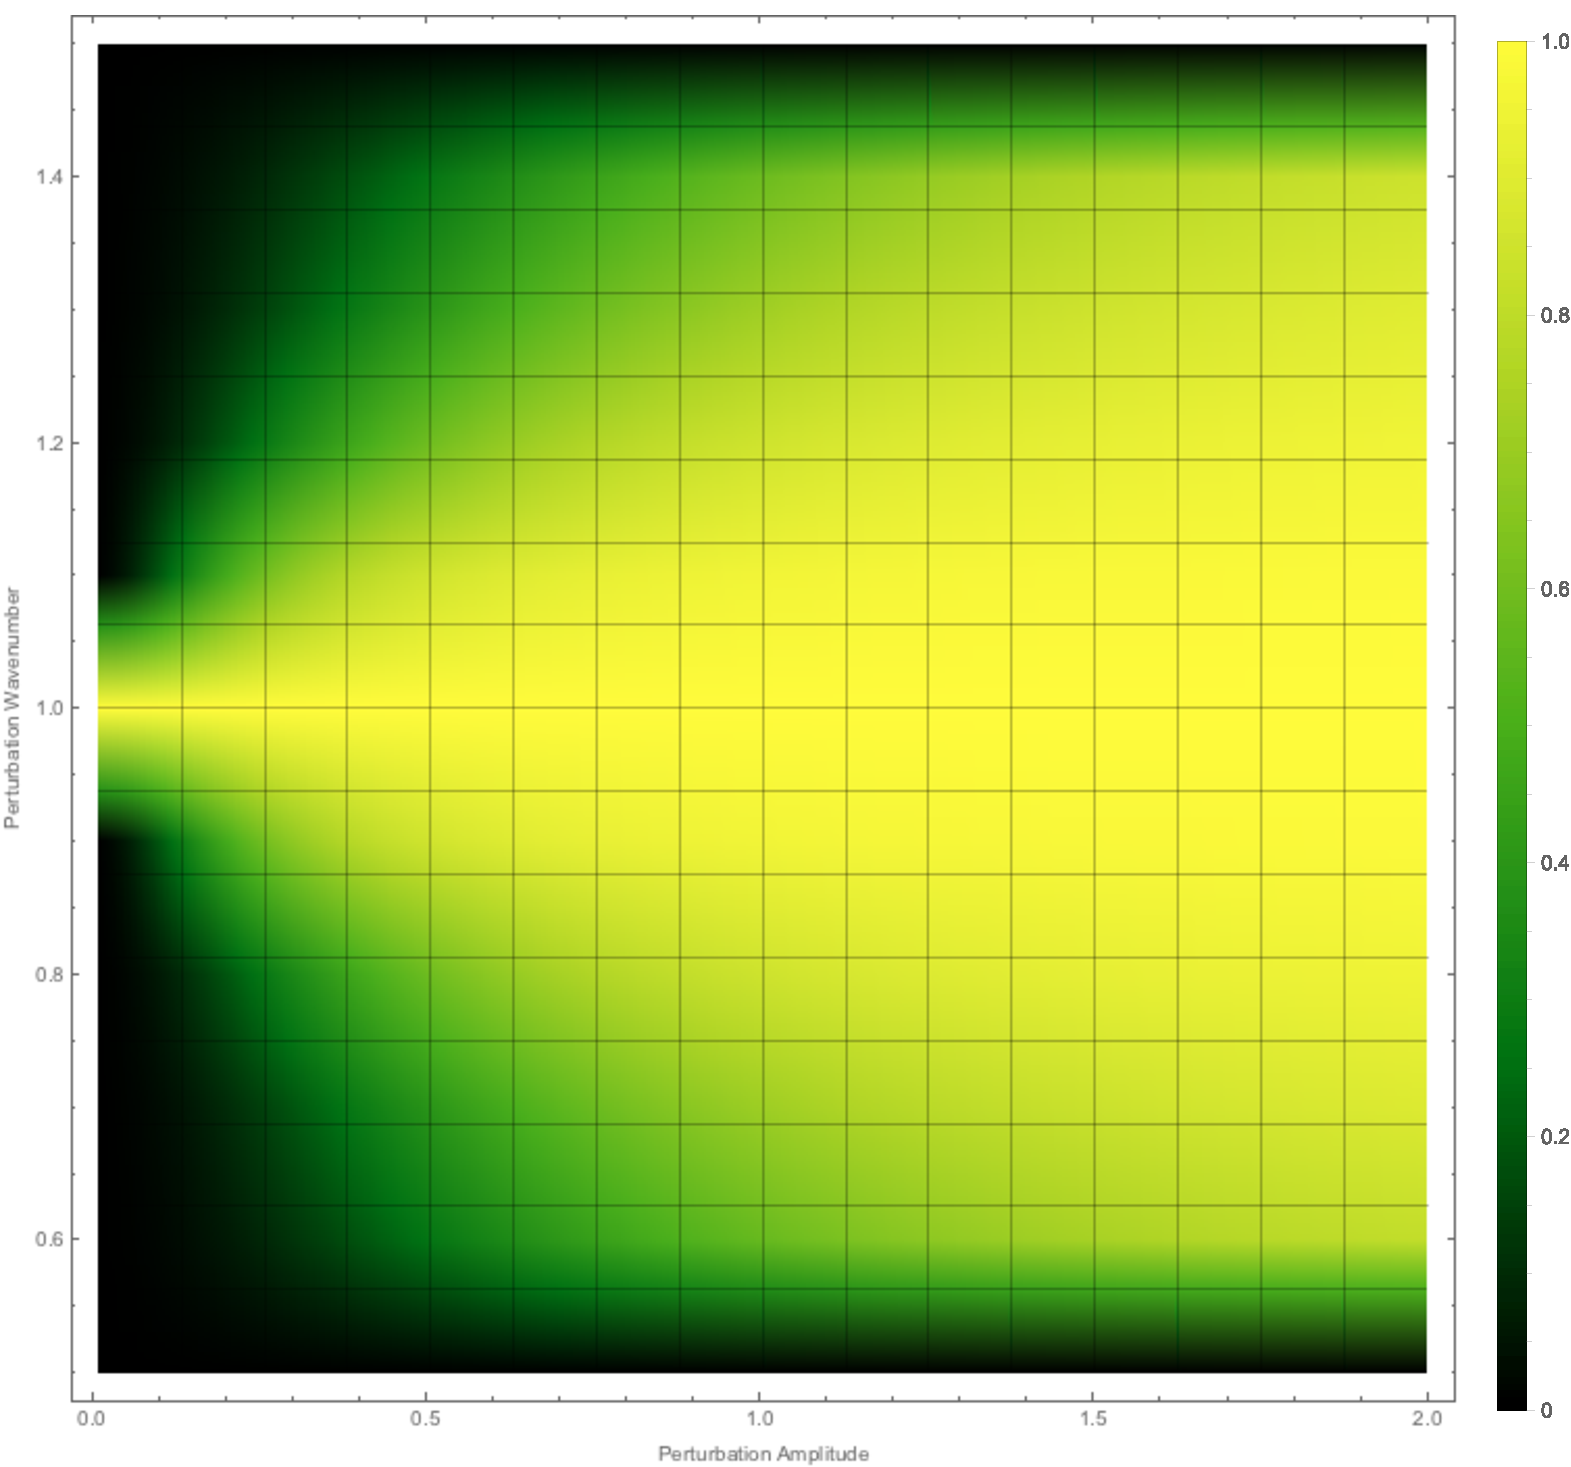
\includegraphics[width=\textwidth]{chapters/assets/rabi/pltPertAmpPertWaveNumTransitionAmp}
%     \caption{Transition probability amplitude at different perturbation amplitude and perturbation wavenumber. Larger amplitudes corresponds to larger resonance width, as another confirmation to Fig.~\ref{chap:matter-sec:single-revisted-fig:resonance-width-jacobi-anger-exp}.}
%     \label{chap:matter-sec:single-revisted-fig:resonance-width-heatmap}
% \end{figure}



\section{\label{chap:matter-subsec:multi-frequency-revisited}Multi-frequency Matter Profile Revisited}


For a multi-frequency matter profile 
\begin{equation}
    \lambda(r) = \lambda_0 + \sum_a \lambda_a \cos (k_a r),
\end{equation}
it is straightforward although a little bit tedious to show that the Hamiltonian in the Rabi basis is 
% the derivation is the same as the derivation for single frequency matter profiles but with more tedious math. The Hamiltonian for neutrino oscillations in multi-frequency matter profile in Rabi basis is
\begin{equation}
    \mathsf H^{(\RR)} = - \frac{\omega_\mm}{2} \sigma_3 - \frac{1}{2} \sum_{ \{n_a\} } A_{ \{n_a\} } 
    \begin{pmatrix}
    0 &   e^{ i K_{\{n_a\}} r }\\
    e^{ -i K_{\{n_a\}} r}  & 0 
    \end{pmatrix},
\end{equation}
% \begin{equation}
%     \mathsf H^{(\RR)} = -\frac{\omega_\mm}{2}\sigma_3 + \begin{pmatrix}
%         0 & h\\
%         h^{*} & 0
%         \end{pmatrix},
% \end{equation}
where $\{n_a\}$ stands for a set of arbitrary integers each associating with a particular Fourier mode, and
\begin{equation}
    K_{\{n_a\}} = \sum_{a} n_a k_a
\end{equation}
and
\begin{equation}
    A_{\{n_a\}} = \tan(2\theta_\mm) K_{\{n_a\}} \prod_{a} J_{n_a} \left( \frac{\lambda_{a}}{ k_{a} } \cos(2\theta_\mm) \right).
\end{equation}
are the wave number and amplitude of the Rabi mode denoted by $\{n_a\}$, respectively. There are potentially many Rabi modes that approximately satisfy the resonance condition
\begin{equation}
    K_{\{n_a\}} = \omega_\mm .
\end{equation}
However, according to the discussion in Sec.~\ref{chap:matter-sec:single-revisted}, the Rabi modes with large $\vert n_a\vert$s have very long oscillation wavelengths and can be ignored even if they are on resonance. The off-resonance Rabi modes with large $\vert n_a\vert$s have very small amplitudes and do not have a significant impact on the resonance either. Therefore, only a finite number of Rabi modes need to be considered for a realistic system.
% To demonstrate the procedure of Jacobi-Anger expansion as well as the technique
% to decompose the problem into simple Rabi oscillations, I adopt the two frequencies
% matter density scenario. The Hamiltonian is described in Eqn.~\ref{eq-hamiltonian-bg-matter-basis-multi-frequency}. The term $h$ becomes
% \begin{equation}
%     h = \frac{\sin 2\theta_\mm}{2} \sum_{a = 1}^2 \lambda_a \sin (k_a r) \prod_{a=1}^2 \sum_{n=-\infty}^{\infty} (-\ri)^n J_n ( \lambda_a \cos 2\theta_\mm/{k_a} ) e^{\ri n k_a r }.
%     \label{chap:matter-subsec:multi-frequency-revisited-eqn:rabi-hamil-off}
% \end{equation}
% The summations and products can be rewritten using the trick,
% \begin{equation}
%     \sum_n a_n \sum_\mm b_\mm  = \sum_{N = -\infty}^{\infty} \sum_{m+n=N} a_n b_\mm = \sum_{N=-\infty}^\infty \sum_{n=-\infty}^{N} a_n b_{N-n}.
%   \label{chap:matter-subsec:multi-frequency-revisited-eqn:multiplication-summation-rule}
% \end{equation}
% For further simplifications of the problem, I follow a rule to sum over a line $m+n=N$ then sum over $N$, which is illustrated in Fig.~\ref{chap:matter-sec:jacobi-subsec:multi-matter-freq-fig:summation-algebra}.
% \begin{figure}[!htbp]
%     \centering
%     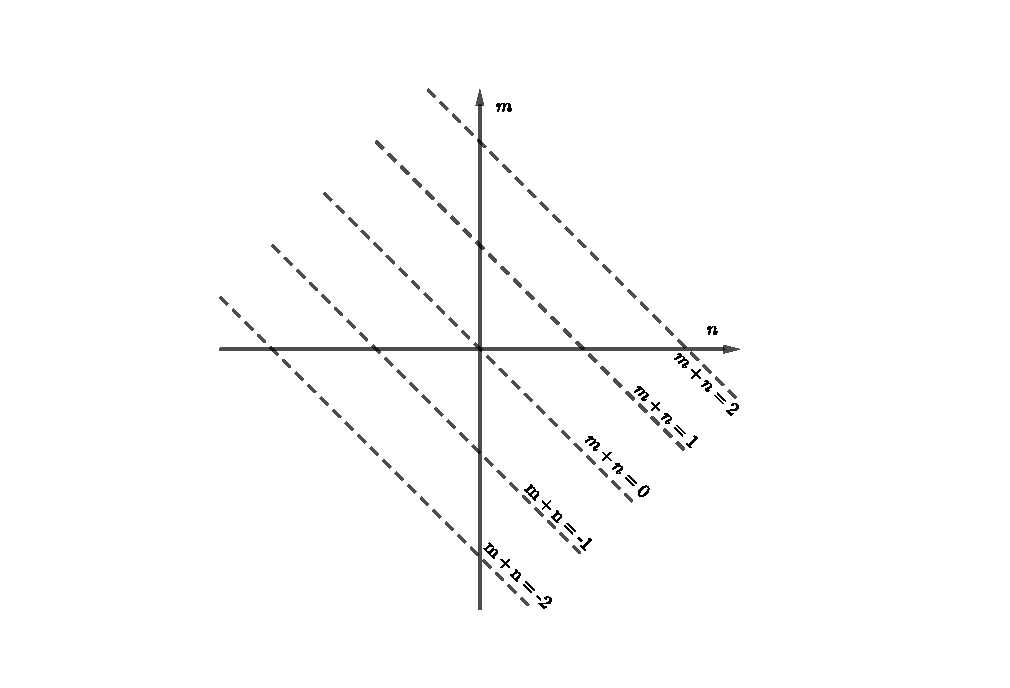
\includegraphics[width=\textwidth]{chapters/assets/rabi/summation-algebra}
%     \caption{Rewrite multiplication of summations into summations only. The horizontal axis is for the summation index $n$ and the vertical axis is for the summation index $m$. The dashed lines are the lines of equal $m+n$.}
%     \label{chap:matter-sec:jacobi-subsec:multi-matter-freq-fig:summation-algebra}
% \end{figure}
% Eqn.~\ref{chap:matter-subsec:multi-frequency-revisited-eqn:rabi-hamil-off} becomes
% \begin{align}
%    h =& \frac{\sin 2\theta_\mm}{2} \sum_{a = 1}^2 \lambda_a \sin (k_a r)  \nonumber\\
%    &\sum_{N=-\infty}^{\infty} \sum_{n=-\infty}^{N} (-\ri)^n J_n ( \lambda_1 \cos 2\theta_\mm / k_1) e^{i n k_1 r } (-\ri)^{N-n} J_{N-n}( \lambda_2\cos 2\theta_\mm /k_2) e^{\ri (N-n)(k_2 r)} \nonumber\\
%    =&\frac{\sin 2\theta_\mm}{2} \sum_{a = 1}^2 \lambda_a \sin (k_a r )  \nonumber\\
%    &\sum_{N=-\infty}^{\infty} \sum_{n=-\infty}^{N} (-\ri)^N J_{n}( \lambda_1\cos 2\theta_\mm / k_1) J_{N-n}(  \lambda_2 \cos 2\theta_\mm /k_2 ) e^{\ri n ((k_1-k_2)r ) + \ri N (k_2 r)}
%    \label{chap:matter-sec:jacobi-subsec:multi-matter-freq-eqn:stimulated-multi-freq-hamiltonian-12-element}
% \end{align}
% I can also rewrite $\sum_{a = 1}^2 \lambda_a \sin (k_a r)$,
% \begin{align}
%    &\lambda_1 \sin(k_1 r ) + \lambda_2 \sin(k_2 r) \nonumber\\
%    = & \frac{\lambda_1}{2 \ri}\left( e^{\ri(k_1 r)} +  e^{-\ri(k_1 r)} \right) + \frac{\lambda_2}{2\ri} \left( e^{\ri(k_2 r)} +  e^{-\ri(k_2 r)} \right).
% \end{align}
% Using the relation Eqn.~\ref{eqn:bessel-function-sum-property}, I can combine the terms and simplify $h$ to
% \begin{equation}
% \end{equation}

% Using the relations of Bessel functions in Eqn.~\ref{eqn:bessel-function-sum-property}, I can decompose $h$ into two terms
% \begin{align}
%     h =& -\sum_{n_1 = -\infty}^\infty \sum_{n_2 = -\infty}^\infty  \frac{\tan 2\theta_\mm}{2} \sum_a n_a k_a \\
%     & J_{n_1} ( \lambda_1 \cos 2\theta_\mm/k_1)  J_{n_2} ( \lambda_2 \cos 2\theta_\mm/k_2)  e^{  \ri \sum_a n_a k_a r } .
% \end{align}

As an example of a matter profile with multiple frequencies, I will consider the castle wall profile
%The arguments that I applied to single frequency matter profile are still valid for multi-frequency matter profiles. For completeness of this section, I will present one example of multi-frequency matter profile. One of the multi-frequency matter profiles that has been well studied is the castle wall matter profile. I can decompose the periodic castle wall matter profile into many Fourier modes and study the interference effect. The potential shown in Fig.~\ref{fig-castlewall-profile-illustration} is defined as,
\begin{equation}
    \lambda(r) = \begin{cases}
\Lambda_1 &\quad \text{if } -\frac{X_1}{2}+nX\le r\le \frac{X_1}{2}+nX, \\
\Lambda_2 &\quad \text{otherwise}, %\frac{X_1}{2}+nX\le r\le \frac{X_1}{2}+\frac{X_2}{2} +n X,
\end{cases}
\label{eq-castle-wall-potential}
\end{equation}
where $n$ is arbitrary integer, $X$ is the period of the potential, and $\Lambda_1$, $\Lambda_2$, and $X_1$ are constants. The parametric resonance condition for the castle wall potential has been derived by E. Akhmedov~\cite{Akhmedov2000}:
\begin{equation}
    \frac{\tan (\omega_{\mathrm m1}X_1/2)}{\tan (\omega_{\mathrm m2}X_2/2)} = - \frac{\cos 2\theta_{\mathrm m2}}{\cos 2\theta_{\mathrm m1}},
    \label{eq-akhmedov-resonance-condition-castle-wall}
\end{equation}
where 
\begin{equation}
    \omega_{\mm i} = \omega_\vv \sqrt{ ( \Lambda_i/\omega_\vv - \cos (2\theta_\vv) )^2  + \sin^2 2\theta_\mm },
\end{equation}
\begin{equation}
\theta_{\mm i} = \frac{1}{2} \arctan \left( \frac{\sin (2\theta_\vv)}{  \cos (2\theta_\vv) - \Lambda_i/\omega_\vv} \right)
\end{equation}
and $X_2 = X_1$. To study the parametric resonance with this particular matter profile, I will decompose the profile into a Fourier series:
% Even though this castle wall problem is analytically solved, the resonance condition Eqn.~(\ref{eq-akhmedov-resonance-condition-castle-wall}) itself is not transparent. In this subsection, we show that such a system is closed related to Rabi oscillations. For illustration purpose, we set the profile to be equal period for the two densities so that $X_1=X_2\equiv X/2$. To show that the neutrino flavor conversions in this castle wall matter profiles is related to Rabi oscillation, we decompose the profile using Fourier series,
\begin{equation}
\lambda(r) = \lambda_0 + \sum_{a=1}^{\infty} \lambda_a \cos\left( k_a  r \right),
\label{eq-castle-wall-fourier-expanded}
\end{equation}
where I have assumed $X_1=X_2 = X/2$,
\begin{align*}
\lambda_0 &= (\Lambda_1 + \Lambda_2)/2, \\
\lambda_a & = \frac{2}{(2a-1)\pi}  (-1)^a  \left( \Lambda_1 -  \Lambda_2 \right),\\
k_a &= (2a-1)k_1, \\
k_1 &= 2\pi/X.
\end{align*}
% The decomposition is visualized in Fig.~\ref{app-chap:convention-sec:fourier-series-eqn:parametric-resonance-castle-wall-fourier-coeff-even}.
As a concrete example, I choose $\Lambda_1 = 0.3\omega_\vv \cos (2\theta_\vv)$, $\Lambda_2 = 0.7\omega_\vv \cos (2\theta_\vv)$, and $X=2\pi/\omega_\mm$. For this particular example, the Rabi mode $\{1, 0, 0, \cdots \}$ is on resonance. In Fig.~\ref{fig-akhmedovOscPlt}, I compared the numerical solution to the full equation of motion and that obtained from the Rabi formula in Eqn.~\ref{app:rabi-system-transition-probability}. They agree with each other very well.


% To calculate the transitions between two mass states of background matter potential $\lambda_0$, we use the background matter basis with respect to $\lambda_0$, in which the transition is zero when varying matter profile vanishes. The Hamiltonian
% \begin{equation}
% \mathsf H^{(\mathrm m)} = - \frac{1}{2}\omega_{\mathrm m} \sigma_3  + \frac{1}{2} \sum_{n=1}^{\infty} \lambda_n \cos 2\theta_{\mathrm m} \cos\left( k_n  r \right)  \sigma_3 - \frac{1}{2} \sum_{n=1}^{\infty} \lambda_n \sin 2\theta_{\mathrm m}  \cos\left( k_n r \right) \sigma_1,
% \label{castle-wall-decomposed-hamiltonian}
% \end{equation}
% determines the transitions between the two background matter states.


% \begin{figure}[!htbp]
%     \centering
%     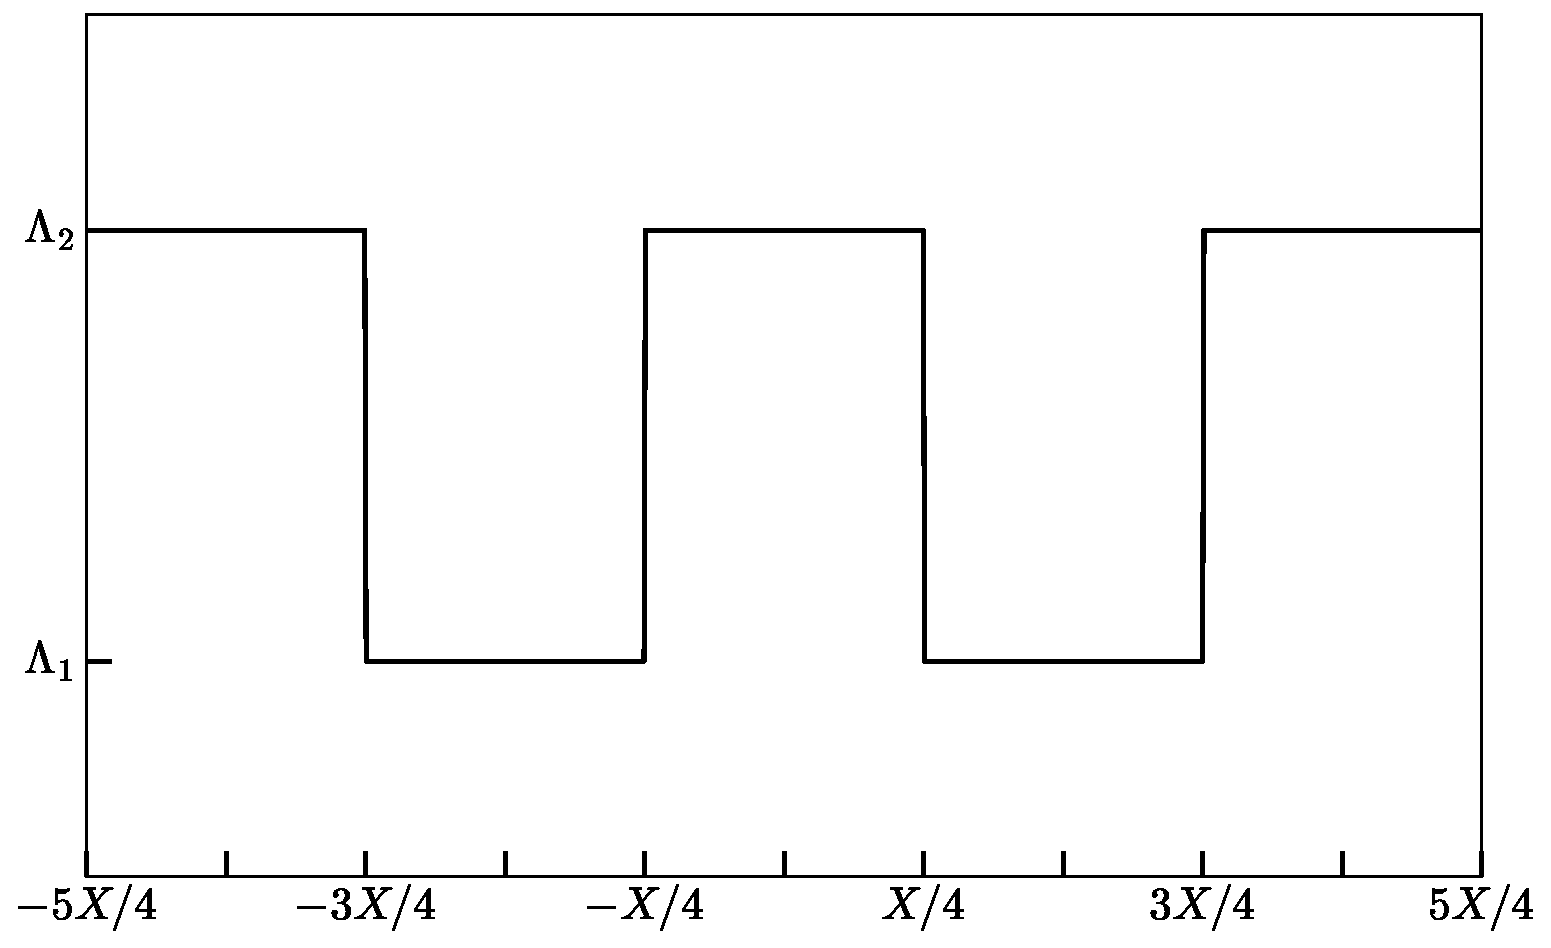
\includegraphics[width=\columnwidth]{chapters/assets/rabi/castlewall-profile}
%     \caption{The castle wall matter potential profile with $X_1=X_2=X/2$. $\Lambda_2 =0.7\omega_{\mathrm v} \cos 2\theta_{\mathrm v} $ \\  $\Lambda_1 = 0.3\omega_{\mathrm v} \cos 2\theta_{\mathrm v}$}
%     \label{fig-castlewall-profile-illustration}
% \end{figure}



% \begin{figure}[!htbp]
%     \centering
%     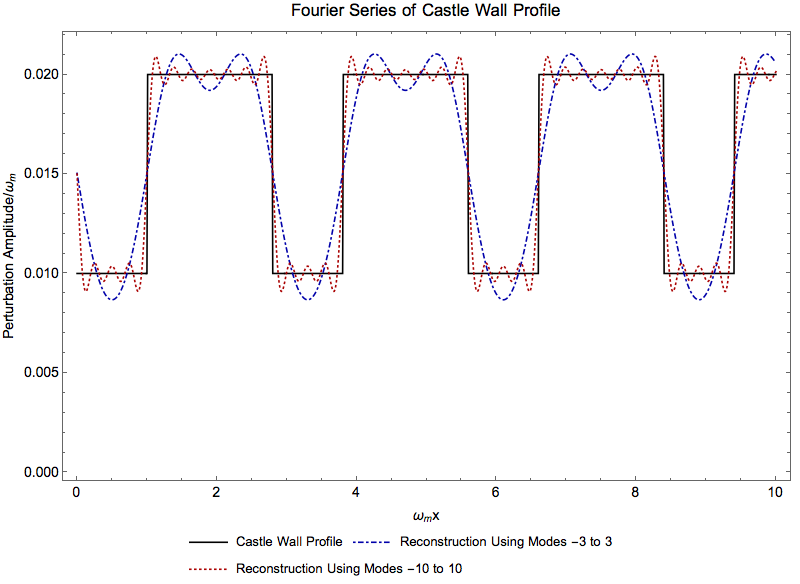
\includegraphics[width=\textwidth]{chapters/assets/rabi/reconstruction-of-castle-wall-0point01-0point02-1-1point8}
%     \caption{Decomposition of castle wall density profile using Fourier modes.}
%     \label{chap:matter-sec:castlewall-fig:decompose-castlewall-fourier}
% \end{figure}


\begin{figure}[!htbp]
        % 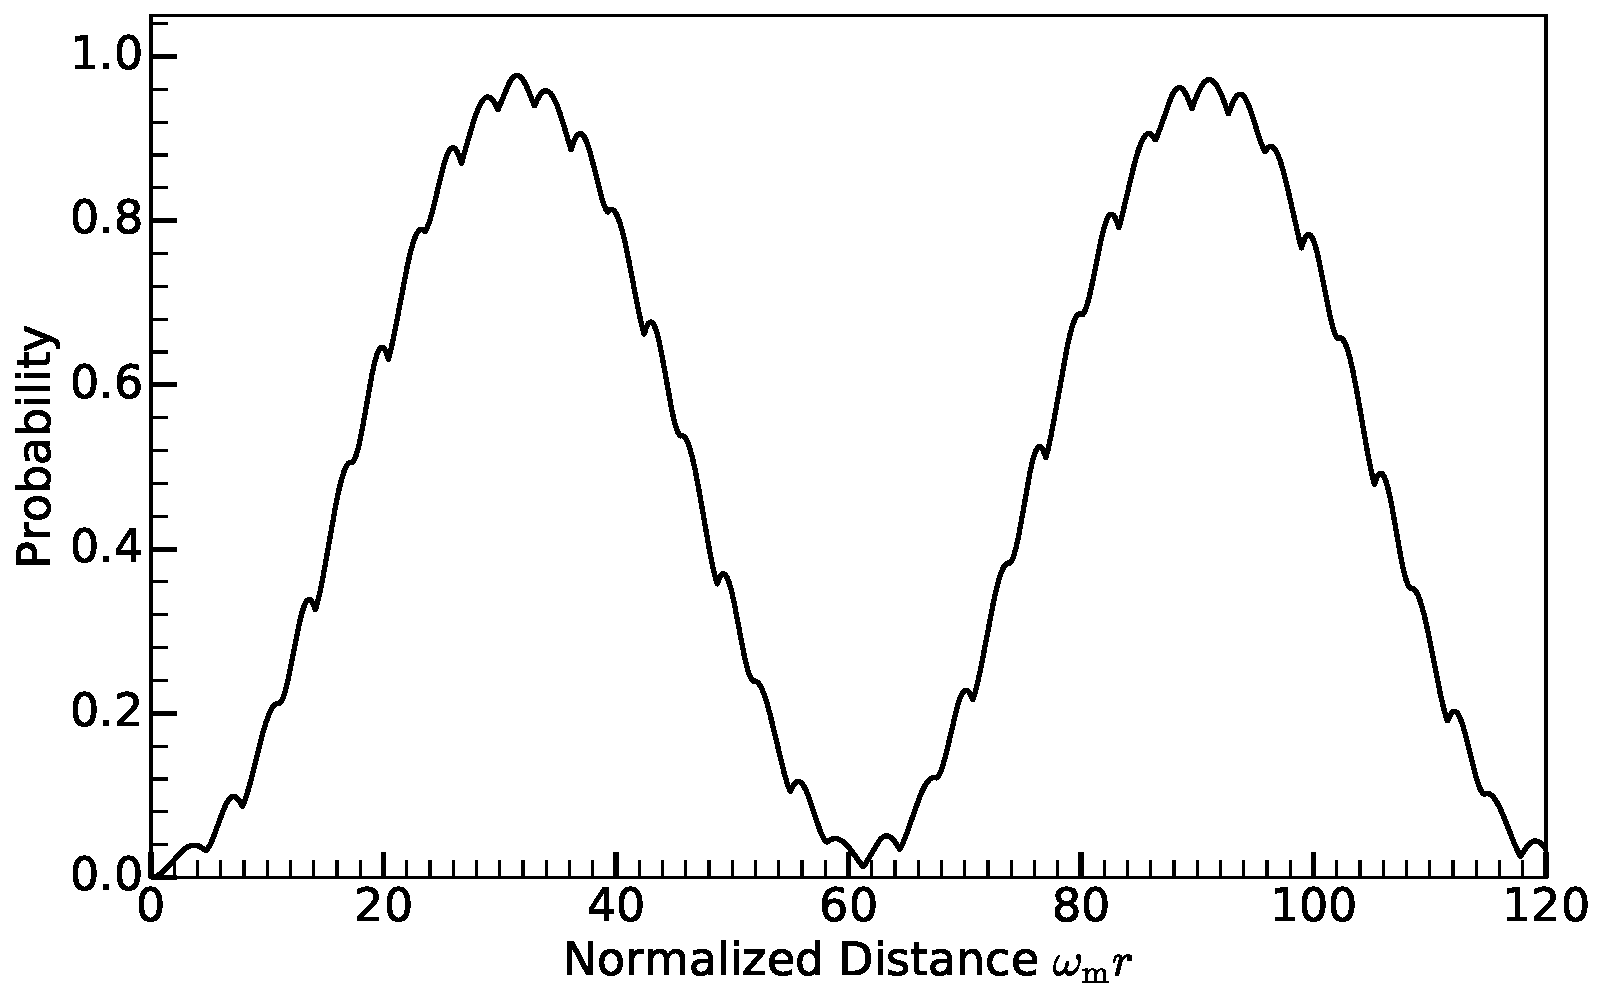
\includegraphics[width=\columnwidth]{chapters/assets/rabi/castle-wall-1}%
        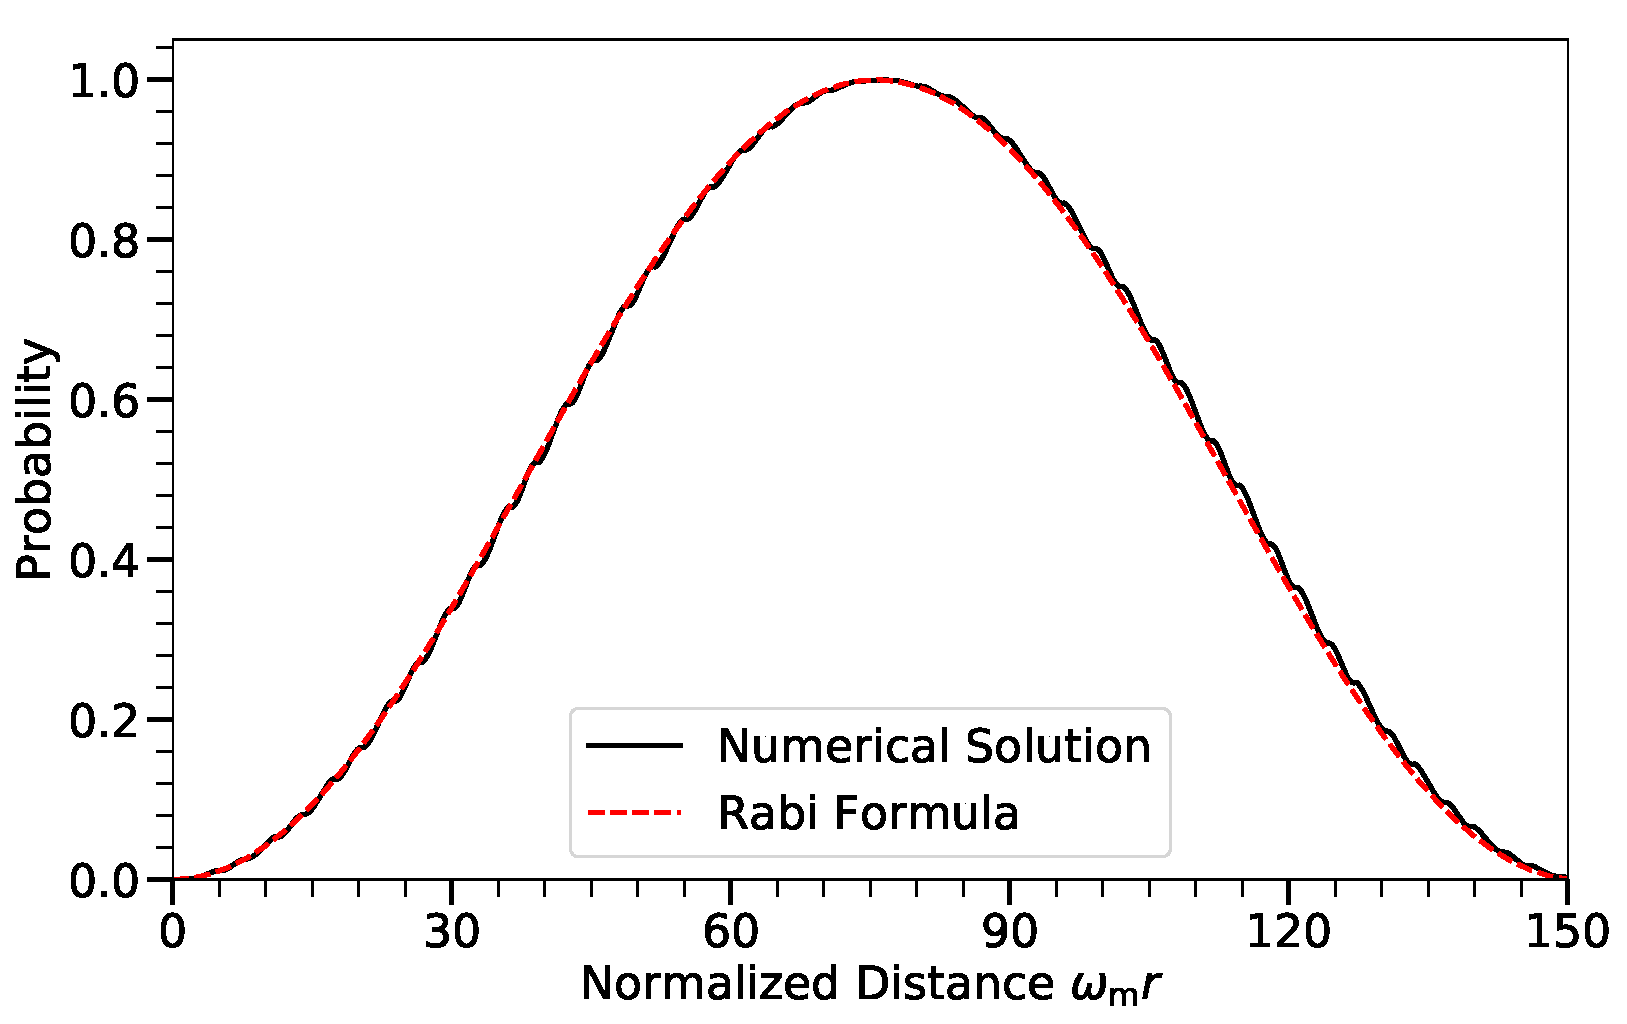
\includegraphics[width=\columnwidth]{chapters/assets/matter/castle-wall-with-legend}%
    \caption{The transition probabilities of neutrino flavor conversion with a castle wall matter profile as functions of distance $r$. The period of the castle wall potential $X$ is chosen that the Rabi mode with wave number $K=1$ is on resonance.
    %to match  base frequency . numerically for $\Lambda_2-\Lambda_1=0.4 \Lambda_0$. During the calculation, the energy of neutrinos is $10\,\mathrm{MeV}$, mass-squared difference is $\delta m^2=2.6\times 10^{-3}\,\mathrm{eV^2}$, and the vacuum mixing angle chosen so that $\sin^2(2\theta_\vv)=0.093$. The background potential $\Lambda_0$ is chosen so that it's half the MSW resonance potential, $\Lambda_0 = \frac{1}{2}\lambda_{\mathrm{MSW}}=\frac{1}{2}\omega_{\mathrm{v}}\cos 2\theta_{\mathrm v}$, and the base frequency is set to $k_0 = 2\pi/X = \omega_{\mathrm{m}}$.
      }
    \label{fig-akhmedovOscPlt}
\end{figure}

In the above example, there are an infinite number of Rabi modes that are on resonance in addition to $\{1,0,0, \cdots\}$. In principle, one should add the amplitudes of all these resonances modes together in calculating the transition probability with the Rabi formula. However, all the Rabi modes that on resonance have very tiny amplitudes except $\{1,0,0,\cdots\}$ (see Table.~\ref{table:castle-wall-relative-detunings-some}), therefore they can be neglected in calculations. There are also an infinite number of Rabi modes that off resonance. In Table.~\ref{table:castle-wall-relative-detunings-some} I listed some of these Rabi modes with the largest amplitudes. One can see that the change to the relative detunings $\RD_{(\{n_a\})}$ of the on-resonance mode $\{1,0,0,\cdots\}$ due to the presence of the mode $\{n_a\}$ are all very small. As a result, they all have very little impact on the neutrino flavor conversion. This explains the agreement between the numerical solution and the result using the Rabi formula in Fig.~\ref{fig-akhmedovOscPlt}.


% The base frequency $k_1$ which is determined by the total period $X$ can be arbitrary. In this example, we choose a $X$ so that the base frequency $k_0$ matches the energy gap $\omega_{\mathrm{m}}$. Even though multiple perturbation frequencies show up in Eqn.~(\ref{castle-wall-decomposed-hamiltonian}), we identify that only the first frequency $n=1$ is the resonance frequency since we are using $k_0=\omega_{\mathrm{m}}$. As an approximation, we drop all other frequencies $n>2$ regarding the fact that they are far from resonance. Thus, similar to single frequency matter profile, the varying $\sigma_3$ terms have limited effects on the transition probabilities in our case, which leads to
% \begin{align*}
%     \mathsf H^{(\mathrm m)} \to & - \frac{1}{2}\omega_{\mathrm m} \sigma_3  - \frac{1}{2} \sum_{n=1}^2\lambda_n \sin 2\theta_{\mathrm m}  \cos\left( k_n r \right) \sigma_1\\
%     \to & - \frac{1}{2}\omega_{\mathrm m} \sigma_3  - \frac{1}{2} \sum_{n=1}^2 A_n \cos ( k_n r) \sigma_1 \\
%     & + \frac{1}{2} \sum_{n=1}^2A_n \cos(k_n r) \sigma_2,
% \end{align*}
% where
% \begin{equation*}
% A_n = \frac{\lambda_n \sin 2\theta_{\mathrm m} }{2} .
% \end{equation*}
% The relative detuning is $0$ if we have only the first mode. However, it becomes
% \begin{equation}
% \RD_1'= \frac{A_2^2}{2\lvert A_1 (\omega_{\mathrm m} - k_2) \rvert},
% \end{equation}
% if we include the second frequency $k_2$. One feature of this Fourier series expanded matter profile Eqn.~(\ref{eq-castle-wall-fourier-expanded}) is that the width of each frequency decreases as the order $n$ increases while the detuning of each frequency increases. We calculate the relative detuning for each frequency
% \begin{equation}
% \RD_n = \frac{\lvert k_n -\omega_{\mathrm m} \rvert}{ \lvert \lambda_n  \sin 2\theta_{\mathrm m}/2 \rvert } = \frac{2(n-1)(2n-1)\pi \omega_{\mathrm m}}{(\Lambda_2 - \Lambda_1)\sin 2\theta_{\mathrm m}}
% \end{equation}
% which is quadratic in $n$ and inversely proportional to $\Lambda_2-\Lambda_1$. We find that all higher frequencies $k_n$ for $n>2$ have very large relative detunings. The neutrino transition probability between the two matter states is shown in Fig.~\ref{fig-akhmedovOscPlt}, where we find the system has almost full transition.

% A more rigorous treatment is to use Jacobi-Anger expansion and find the Rabi modes, where we find that the mode that corresponds to single frequency $k_1$ dominates and all other modes have little destruction effect on it. Quantitatively, higher orders leads to smaller width $A_{\{n_i\}}$ yet larger detuning $\sum_{n} nk_n-\omega_{\mathrm m}$, which renders a smaller effect on the resonance mode $\{1,0\}$, since the effect is evaluated as Eqn.~(\ref{app:chap:matter-eq:relative-detuning-changed}).
% Table~\ref{tab-q-values-each-mode} lists the first few smallest relative detunings of Fig.~\ref{fig-akhmedovOscPlt}. The second column is the relative detuning of the corresponding mode, while the third column is the relative detuning of mode $\{1,0\}$ with the energy gap shift effect of the corresponding mode.



% Find the data in MMA file `akhmedov-parametric-resonance.nb`
% {0., 6129.81, 20432.7, 42908.7}
% {0., 5.99981, 19.9994, 41.9987}

% \begin{table}
% \centering

% % \begin{ruledtabular}
% \begin{tabular}{lll}
% \hline
%  $\{n_1,n_2\}$ &  $\RD$ & $\RD'_{\{1,0\}}$   \\
% \hline
%  $\{1,0\}$ & $0$ &  - \\
%  $\{-1,0\}$ & $48$ &  $1.0\times 10^{-2}$ \\
%  $\{0,1\}$ & $1.5\times 10^2$ &  $1.1\times 10^{-3}$  \\
%  $\{2,0\}$ & $2.4\times 10^{2}$ & $2.0\times 10^{-4}$ \\
%  \hline
% \end{tabular}
% % \end{ruledtabular}
% \caption{\label{tab-q-values-each-mode}Relative detuning of each frequency.}
% \end{table}

\begin{table}
    \centering
    % \begin{ruledtabular}
    \setlength\tabcolsep{10pt}
    \begin{tabular}{llll}
    \hline
    \hline
     $\{n_a\}$ & $A_{\{n_a\}}/A_{\{1,0,0,\cdots\}}$  & $\RD_{\{n_a\}}$ & $\Delta \RD_{(\{n_a\})}$  \\
    \hline
    $\{-2, 1, 0,\cdots\}$ & $5.4\times 10^{-4}$ & 0 &  - \\
    $\{-1, -1, 1,\cdots\}$ &  $4.3\times 10^{-5}$ & 0 & - \\
    $\{0, 2, -1,\cdots\}$ & $2.4\times 10^{-6}$ & 0 & - \\
    \hline
     $\{-1,0, 0, \cdots\}$ & $1$ & $48$ &  $1.0\times 10^{-2}$ \\
     $\{0,1, 0, \cdots\}$ & $0.33$ & $1.5\times 10^2$ &  $1.1\times 10^{-3}$  \\
     $\{2,0, 0, \cdots\}$ & $1.3\times 10^{-3}$ & $2.4\times 10^{2}$ & $2.0\times 10^{-4}$ \\
     \hline
     \hline
    \end{tabular}
    % \end{ruledtabular}
    \caption{\label{table:castle-wall-relative-detunings-some}The amplitudes and relative detunings of a few Rabi modes $\{n_a\}$ and the changes to the relative detunings of the on-resonance modes due to these Rabi modes if they are off-resonance.}
\end{table}
%%%%%%%%%%%%%%%%%%
%%% Using data from Mathematica notebook: akhmedov-parametric-resonance.nb


\section{\label{chap:matter-sec:conclusions}Summary}

In this chapter, I have shown that the flavor conversion of a neutrino can be greatly enhanced when it propagates through a oscillatory matter profile when certain resonance conditions are satisfied. This derivation is done from the perspective of Rabi oscillations and is much more physically intuitive than the original derivation by J. Kneller et al. in references~\cite{Kneller2013, Patton2014}. I have shown that, although there can exist an infinite number of Rabi modes that approximately satisfy the resonance condition, only a few of them need to be considered for a real system. I have also derived a criterion when an off-resonance Rabi mode may significantly affect the resonance. Using this criterion I have shown that only a few of the infinite set of off-resonance Rabi modes may contribute to neutrino flavor conversion. Although I have assumed small perturbations on top of a constant matter profile, this approach can be applied to a matter profile with perturbations on top of a smoothly varying background density as have been done by K. Patton et al. in reference~\cite{Patton:2014lza}. This result maybe applicable to the regions in a star where the matter density fluctuates. There can also exist a turbulent matter distribution behind the shock in a core-collapse supernova where this result maybe applicable. However, the large neutrino fluxes inside a supernova core may have an even larger impact neutrino oscillations which we will consider in the next chapter.

% The solar neutrinos behave very differently from lab experiments since the Sun provides a high matter density lab which can not be built on the Earth. What's even more exotic, in a supernova explosion, $10^{58}$ neutrinos are released from the proto-neutron star, which is of radius $10\mathrm{km}$, in a few seconds. The huge number density of neutrinos and large density of matter both change the neutrino oscillations dramatically. The matter effect in supernova is also much more complicated than MSW for solar neutrinos since the rich distribution of matter density and high speed motion. In addition to matter effect, neutrino neutrino interaction will be very efficient because of the high neutrino number density.

% Apart from the emission of neutrinos from nuclear reactions of electron capture and positron emission in the solar interior, supernova environment also gives rise to Bremsstrahlung pair neutrino production, electron-positron neutrino pair production, which brings all three flavors and also anti-neutrinos into the spectra. However, even the with the presence of intensive interaction between neutrinos and the leptons and hardrons, which thermalize the neutrinos in the supernova core, the neutrino spectrum escaping from the supernova core is not completely Fermi-Dirac distribution. Nonetheless, it is possible to parametrize it using nominal Fermi-Dirac distribution,\cite{ysuzuki2004}
% \begin{equation}
% f(E)\propto \frac{E^2}{1+\exp ( E/kT - \mu )}.
% \end{equation}
% Some numerical results show that there is a deviation from this Fermi-Dirac distribution~\cite{Totani1998,Keil2003}. Meanwhile, Keil Mathias and Georg Raffelt showed that it is good enough to approximate the neutrino spectrum from supernova in Monte Carlo simulations using the so called "alpha fit",
% \begin{equation}
% f(E)\propto E^\alpha \exp\left( -(\alpha+1)\frac{E}{\langle E\rangle} \right),
% \end{equation}
% where $\langle E\rangle$ is the average energy, or the first moment of energy. The values from Monte Carlo simulations falls into the range $\alpha = 2.5\sim 5$,
% which clearly shows the spectra are pinched. It's a hint that the detection of deviation from nominal Fermi-Dirac distribution will show evidence of core-collapse information.


% % \begin{figure}
% % \centering
% % 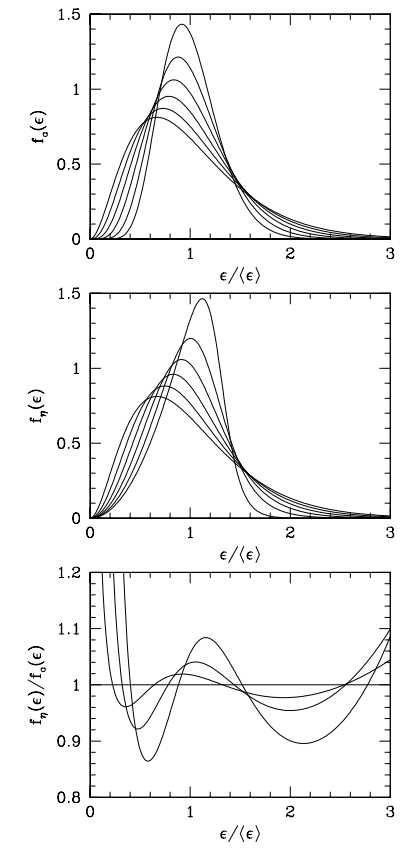
\includegraphics[width=\columnwidth]{chapters/assets/solar/neutrino_spectra_sn_simulations.png}
% % \caption{Alpha fit and nominal Fermi-Dirac fit comparison. The top panel is alpha fit results while the middle panel is from nominal Fermi-Dirac distribution fit. The broadest curve are for $\alpha=2$. The width $w=\sqrt{\langle E^2 \rangle - \langle E\rangle^2}$ decrease 10\% for each curve. The bottom panel is the ratio of the two fit functions.}
% % \label{fig:neutrino_spectra_sn_simulations}
% % \end{figure}


% Even though we understand solar neutrinos well, the neutrino oscillations of supernova explosions are not so to our complete knowledge. The flavor content is subject to the solution to the neutrino oscillations. Phenomena such as spectral split due to neutrino-neutrino interaction and matter effect reshape the neutrino spectra significantly. That being said, more research on supernova neutrinos, especially supernova neutrino oscillations is critical to understand supernova explosion mechanisms, as well as future observation of supernova neutrino data.


% In conclusion, we have provided an interpretation for neutrino flavor conversion in fluctuating matter with the help of Rabi oscillations. The work provided two different points of view that is related to Rabi oscillations.

% The first point of view was to interpret the neutrino flavor conversions in background matter basis. In this basis, matter density fluctuations will introduced a fluctuation part to the diagonal elements of the Hamiltonian, which means that the energy gap is fluctuating if we draw analogy between this Hamiltonian and the Hamiltonian of Rabi oscillations. For neutrino flavor conversions in a single frequency matter profile, the neutrino flavor oscillations becomes large when the matter fluctuation frequency is close to the energy gap, which is the resonance condition. We anticipated that the fluctuations of energy gap have limited effects on neutrino flavor conversions under this resonance condition. Thus the matter fluctuation only works as a pure flipping field that converts neutrinos from one flavor to another.

% As we added more frequencies of matter density fluctuations, the neutrino flavor conversions becomes nontrivial due to the interferences between the difference matter profile frequencies. To quantify the interference between different Rabi oscillation modes, we defined relative detuning which describes how off-resonance a Rabi oscillation is. In the case of single frequency Rabi oscillations, the relative detuning becomes $0$ under the resonance condition. As a second frequency is added to the oscillations, the energy gap is shifted due to this new frequency. A measure of the interference effect is to consider the relative detuning of the first frequency which is at resonance, under the shifted energy gap. Numerical results verified this conjecture. With the interference mechanism, we revisit the single frequency matter profile neutrino oscillations.

% Another view is to switch to a basis where the neutrino oscillations Hamiltonian is decomposed into infinite Rabi oscillations. Equivalently speaking, the oscillations are consequences of superposition of Rabi oscillations, which we call modes of oscillations. This view was applied to emphasis the approximations that the change of energy gap due to matter fluctuation can be neglected under resonance condition in the previous background matter basis.
